\chapter{Design of the \hisparc experiment}
\label{ch:experiment}

\subsection{Design criteria}

In \cref{sec:air-shower-physics} the development of EAS is explained. The definition of the shower front is given and its characteristics. Showers produce a high density of particles near the shower core. The density steeply decreases with increasing distance to the core. Showers of higher energy produce an overal higher density. Given an expected particle density the probability of detecting a certain number of particles is given by the Poisson distribution [$P_k$]. This assumes the detectors are \SI{100}{\percent} efficient at detecting charged particles. The important probability is the probability of not detecting any particle given a particle density [$P_0$]. Which gives the probability of detecting at least one particle [$1-P_0$].

Background radiation includes low energy showers which produce only a couple muons at ground level, to few to effectively detect in multiple detectors. At least two detectors need to detect the shower to distinguish it from the background. This makes the probability of detecting at least a particles in both detectors simultaneously [$P^2$], assuming the core distance is equal for both detectors. There is a lower energy threshold where the probability of detecting the shower becomes very low. This will depend on the size of and distance between the detectors.

To be able to fully reconstruct the direction of an air shower at least three detection points are required. This can either be achieved by a single station with three or more detectors (short distances), or by combining detections from multiple stations (larger distances). The distance between the detection points is one of the variables that determines the accuracy of the direction resolution. The other variable is the accuracy of the time differences between the detections. For direction reconstruction within a station the distances between the detectors will be small, which means that the timing resolution needs to be good. Using a 3-detector station the probability of detecting at least one particle in each becomes [$P^2$], a for a n-detector station this becomes [$\sum_{k=3}^{n} (^n_k) P^k P_0^{n-k}$].

Making detectors larger makes them more likely to detect particles. The downside is that the detector becomes less easy to handle, more expensive, efficiency uniformity may decrease, and saturation might occur sooner. A good balance needs to be determined. The experiment is meant to be accessible for high schools, the detectors need to be fairly easy to handle. If the detectors would be placed inside schools the floor/roof material might affect the detections. In order to have enough space to place the detectors the most obvious location would be on the roof. If the detectors are outside proper protection from weather effects need to be considered.


\section{The \hisparc experiment}

The \hisparc experiment detects cosmic-ray induced air showers by sampling the shower front as it reaches ground level. It is important to make distinctions between different layers of the experiment. Each `layer' will be described thoroughly in the next sections.

Scintillator detectors sample parts of the EAS, detecting charged particles as they pass through the detector. The detectors are described in \cref{sec:detector-design}.

The time and place correlation of particles belonging to the same EAS makes it possible to distinguish them from the background radiation. The particle density gives indications to the size of and distance to the shower. The readout electronics records the strength and arrival time of the signals in the detectors. Detection with multiple detectors is needed to veto the background. Multiple detectors can be connected to the readout electronics which also contain a coincidence trigger. A simple station to detect air showers requires two detectors. Using more than two detectors allows for the reconstruction of some properties of the air shower. Two different station setups have been devised, one with two detectors and one with four. The four detector station is more expensive, but allows for the reconstruction of more shower parameters by itself. The readout and trigger electronics that make the station are described in \cref{sec:station-design}.

By combining the measurements of multiple stations more accurate reconstructions can be made, because more detection points are then used. The time synchronization is done via \gps. Together all stations form the \hisparc network, which is described in \cref{sec:network-design}.

\begin{figure}
    \centering
    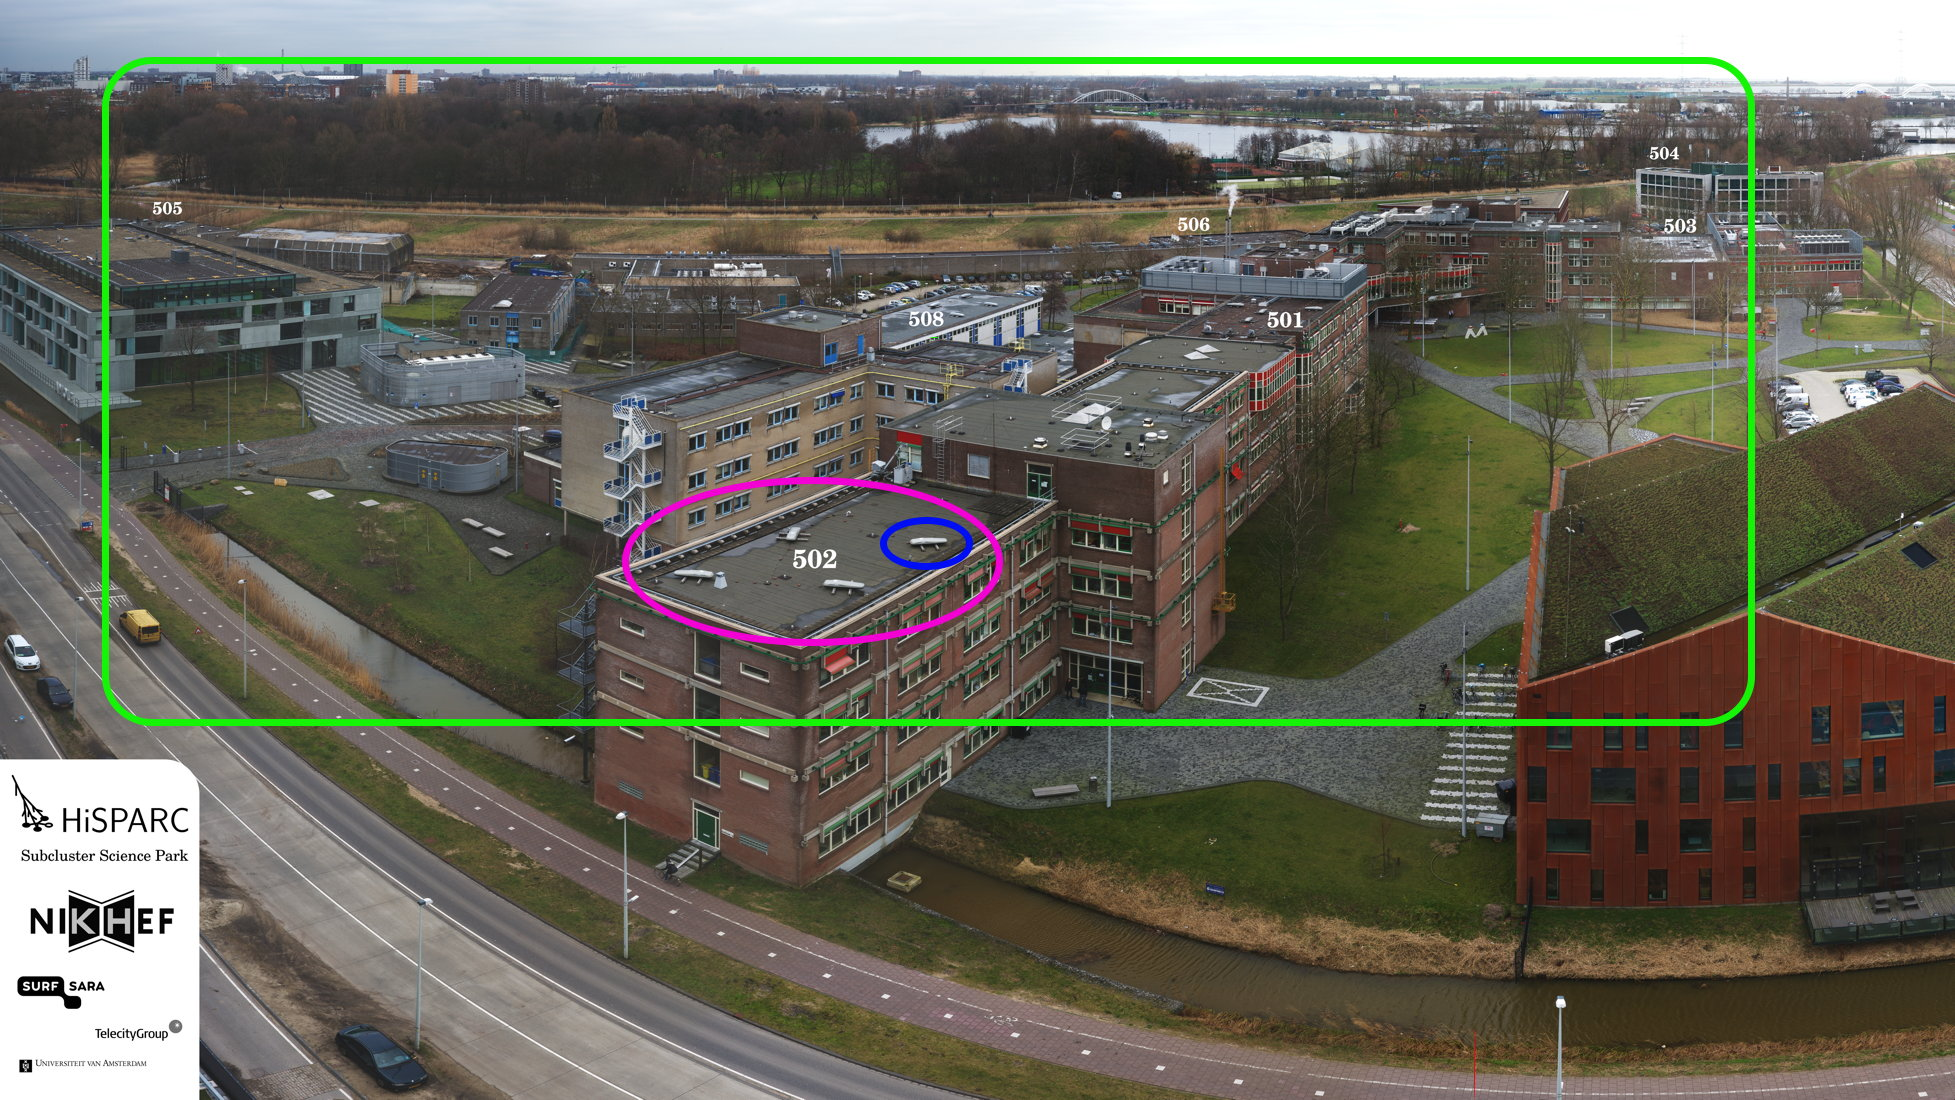
\includegraphics[width=0.6\textwidth]
                    {plots/experiment/ADL_151373_151429_layers}
    \caption{The Science Park cluster. The blue ellipse indicates a single detector. The pink region indicates a single detector stations. The green region encompasses multiple stations (not the entire \hisparc network).}
    \label{fig:sciencepark-layers}
\end{figure}


\section{Detector design}
\label{sec:detector-design}

Scintillators have been chosen as detection material. This is a relatively cheap material with high reliability and good efficiency. The size is chosen such that the number of background particles does not become to high, which maintaining handleability. The size also works well with the choice for the outer case, namely, roof boxes (in Dutch generally referred to as `ski box'). These can be securely fastened and are designed to withstand all kinds of weather.

The scintillator detector consists of two main components which perform the detection. The scintillator, which emits light when charged particles pass through it, and the Photomultiplier tube (PMT) which converts the scintillation photons into an electric signal. The size of detectors affects the probability of detecting a particle given a particle density.

The scintillator is a parallelepiped/sheet of \SI[product-units=power]{100 x 50 x 2}{\centi\meter} made from BC-408 \cite{bc408}. The BC-408 material was chosen for its good timing properties and light output for charged particles.

The photomultiplier tube \cite{et:pmt} is a compact \SI{29}{\milli\meter} diameter PMT. The photomultiplier tube has a front window with a photocathode, when this is hit by a photon an electron can be knocked free. The electron is then pulled along electric field lines which direct it to a dynode. The electron will cause multiple electrons to be emitted from the dynode, these electrons are then pulled to the next dynode, which has a higher positive potential, here again more electrons will be released. A typical PMT has 13 dynodes. At the end the electrons fall on the anode which is connected to the readout.

Besides these the detector construction consists of several other components. An isosceles triangle light guide, which is glued to the scintillator using Optical Cement (\cite{bc600}). A little adapter piece (same material as light guide) is attached to the square end of the triangle with Optical Cement and the round window of the \pmt with optical tape. This construction is wrapped in thin, \SI{30}{\micro\meter}, aluminium foil with patches of thicker, ??, aluminium foil at the corners of the scintillator, to prevent the sharp edges from piercing the thin foil. This is then wrapped in thick, ??, light tight black pond foil to keep light out and protect the aluminium foil from outside influences.

\begin{figure}
    \centering
    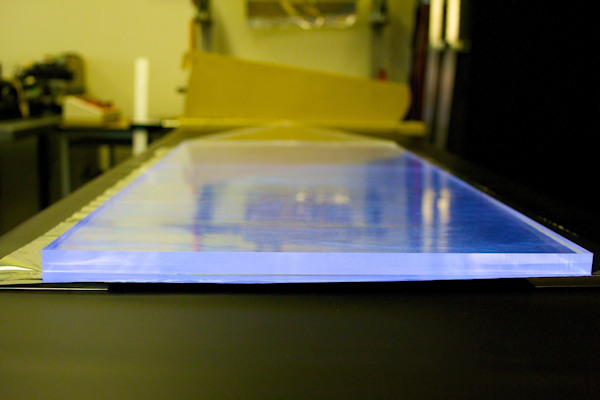
\includegraphics[width=.6\textwidth]{plots/experiment/ADL_115651}
    \caption{Detector in the process of being assembled. Scintillator with the lightguide attached laying on the Aluminium foil and pond foil in which it will be wrapped.}
    \label{fig:scintillator}
\end{figure}


- Add figure; timing scintillator


\subsection{Photo multiplier}

The PMT is used to convert the optical signal from the scintillator to an analog/electrical signal. The PMT must amplify the signal to be much higher than the noise level in the readout electronics.

typical n photons per particle, Quantum efficiency, gain, gain vs time

An alternative for PMTs might be Silicon based sensors (pixels/chips). However, silicon pixels these are not as thermally stable as PMTs. The temperature in a \hisparc skibox can fluctuate over \SI{30}{\degreeCelsius} in a day. The voltage on such (avalanche) chips needs to be controlled carefully to keep them performing optimally. Multi-pixel photon counters (MPPC) have been tested and compared to PMTs \cite[Chapter~3.4]{lio2011} and \cite[Chapter~3.6]{lio2010}. The MPPC have a smaller collection area, smaller temperature range (require cooling?), and increased complexity when using multiple (for increased area/reduced dark counts) MPPC. The conclusion is that at that time the MPPC are not yet ready for use in \hisparc.

The PMTs are attached to the detector with optical tape, allowing them to be replaced easily. breaking index?

Nikhef designed high-voltage voltage-divier circuit.
Cockcroft-Walton voltage multiplier circuit.
High linearity?

There are several types of \pmt being used in the \hisparc experiment. Most established stations used \pmts that were fully created by outside manufacturers. Because of reasons outlined in \cref{sec:detector-durability} a new \pmt power supply has been developed by the Electronics department at \nikhef. The final design is shown in \cref{ch:pmt_design}.



\subsection{Signal response}

A particle is detected if it passes through our detector and leaves some energy behind. These detections end up as a digitized list of numbers with a timestamp. However, before a particle signal ends up in its digital form it passes through the various parts of the detector. Not all parts perfectly transport the particle signal. These effects, which prevent the detector from having perfect timing and particle counting will be outlined. These also serve as probability distributions that are used in detector simulations.


\subsection{Energy loss and light production}

Particles loose energy in the detector because of interactions with the polyvinyltoluene in the scintillator. Ionization and Bremsstrahlung and the main sources of energy loss for energetic charged particles (electrons, muons). The energy is transferred to anthracene molecules which emit light that

This formula gives the stopping power, the amount of energy lost by the particle per \si{\gram\centi\meter\square} of the material it passes through. However, the interactions in which the particles loose energy is a statistical process, so the energy loss is not a fixed number but a distribution.

(figure of energy loss in scintillator)

The scintillator is \SI{2}{\centi\meter} thick, however, most particles have a longer path through the detector because they enter it at an angle. The path can be shorter if the particle passes through one of the edges of the scintillator, but due to the large area of the detector relative to its thickness the chance of that happening is low. The amount of energy deposited by the particle going through the detector is described by the Bethe-Bloch formula.

The light emitted along the path of the particle is transmitted in random directions. Depending on the angle at which the emitted photons hit the outer edges of the scintillator there is a chance that they will be reflected back or leave the scintillator. The entire detector is wrapped in aluminium foil to reflect those photons back into the scintillator. To detect the photons they need to hit the windows of \pmt. To get to the \pmt they need to pass from the scintillator through a layer of optical glue, the light guide, another layer of optical glue, a small piece of light guide, and finally a layer of optical tape to reach the \pmt. During this many photons will be reflected a number of times. For \SI{1}{\mip} approximately 30000 photons [check.] are emitted, most will not make it to the \pmt.

A 2D Monte Carlo simulation performed by Jos Steijger which tracked photons from emission until they either reach the \pmt or leave the detector (ignoring the aluminium foil) gives transmission efficiency information at any location in the scintillator.

According to the specifications the amount of light produced in a scintillator as a function of temperature should be constant between \SI{-60}{\degreeCelsius} and \SI{20}{\degreeCelsius}. At \SI{60}{\degreeCelsius} the light output is decreased by \SI{5}{\percent} relative to the output at \SI{20}{\degreeCelsius}. Temperature in a skibox can rise above the local outside temperature when the sun shines upon it. Temperature loggers have measured differences of over \SI{10}{\degreeCelsius} above the local outside temperature. Rarely but sometimes the temperature in the Netherlands can reach \SI{40}{\degreeCelsius}, so on such occasions the efficiency of the scintillator might be \SI{3.75}{\percent} below nominal. Given the rare occurrence of such extremely high temperatures and the small effect this is ignored in the analysis and simulations.


\subsection{\mip/MPV}

The number of particles in a detector are determined by the pulse integral, the integrated signal of the \pmt recorded by the \adc. When making a histogram of all pulsintegrals this will not show discrete values for the number of particles in each detection but a continuous distribution. There is overlap in the pulse integrals from one particle and the pulse integrals from two particles. The pulse integral histogram does peak at a certain value, this is the most probable value for the pulse for one particle, since it dominates the histogram. The value at which this peak occurs is called the Most Probable Value (MPV).


\subsubsection{Gammas}

\todo{Signals in detector from gammas}

Energetic photons can also deposit energy in the scintillator due to Compton scattering and pair creation. However, the cross sections for these interactions is very low. A \SI{1}{\MeV} photon  has a mean free path greater than \SI{10}{\centi\meter}, which increases further for higher energy photons, see fig [By Jos/Tom]. Despite the low detection chance, the large number of photons in an air shower makes them statistically relevant.


\subsection{Detector timing}

\subsubsection{Fluorescence}

rise time - 0.9 ns, decay time - 2.1 ns, pulse width 2.5 ns.

\todo{deexcitation fast (2.1 ns), slow phosphorescence
      (14.2 ns), ratio?}


\subsubsection{Light transport and \pmt efficiency}

Similar to the model that predicts the signal transport efficiency in
the scintillator a models that calculates the transport time of these
photons has been made. Quantum efficiency of the \pmt causes not every
photon reaching the \pmt to produce a photoelectron. Multiple photons
are required for the \pmt to produce a significant signal that the
\hisparc electronics triggers. The model tracks the time at which the
15th photon producing a photoelectron reaches the \pmt. 15
photoelectrons are required for a signal of \SI{70}{\milli\volt} (high
threshold).

In the simulations for each particle within the bounds of the
scintillator a number is taken from this distribution simulate the
transport time of each particle.

\begin{figure}
    \centering
    % \usepackage{tikz}
% \usetikzlibrary{arrows}
% \usepackage{pgfplots}
% \pgfplotsset{compat=1.3}
% \usepackage[detect-family]{siunitx}
% \usepackage[eulergreek]{sansmath}
% \sisetup{text-sf=\sansmath}
% \usepackage{relsize}
%
\pgfkeysifdefined{/artist/width}
    {\pgfkeysgetvalue{/artist/width}{\defaultwidth}}
    {\def\defaultwidth{ .67\linewidth }}
%
%
\begin{sansmath}
\begin{tikzpicture}[
        font=\sffamily,
        every pin/.style={inner sep=2pt, font={\sffamily\smaller}},
        every label/.style={inner sep=2pt, font={\sffamily\smaller}},
        every pin edge/.style={<-, >=stealth', shorten <=2pt},
        pin distance=2.5ex,
    ]
    \begin{axis}[
            width=\defaultwidth,
            %
            title={  },
            %
            xlabel={ Transport time [\si{\nano\second}] },
            ylabel={ Counts },
            %
            xmin={ 1 },
            xmax={ 8 },
            ymin={ 0 },
            ymax={  },
            %
            xtick={  },
            ytick={  },
            %
            tick align=outside,
            max space between ticks=40,
            every tick/.style={},
        ]

        

        

        
            
            % Draw series plot
            \addplot[no markers,gray,const plot] coordinates {
                (1.0, 0.0)
                (1.1, 0.0)
                (1.2, 1.0)
                (1.3, 3.0)
                (1.4, 2.0)
                (1.5, 4.0)
                (1.6, 3.0)
                (1.7, 2.0)
                (1.8, 5.0)
                (1.9, 19.0)
                (2.0, 22.0)
                (2.1, 26.0)
                (2.2, 34.0)
                (2.3, 58.0)
                (2.4, 78.0)
                (2.5, 123.0)
                (2.6, 201.0)
                (2.7, 296.0)
                (2.8, 414.0)
                (2.9, 445.0)
                (3.0, 435.0)
                (3.1, 460.0)
                (3.2, 552.0)
                (3.3, 579.0)
                (3.4, 304.0)
                (3.5, 196.0)
                (3.6, 198.0)
                (3.7, 185.0)
                (3.8, 191.0)
                (3.9, 193.0)
                (4.0, 165.0)
                (4.1, 203.0)
                (4.2, 177.0)
                (4.3, 218.0)
                (4.4, 239.0)
                (4.5, 199.0)
                (4.6, 205.0)
                (4.7, 192.0)
                (4.8, 218.0)
                (4.9, 165.0)
                (5.0, 230.0)
                (5.1, 183.0)
                (5.2, 216.0)
                (5.3, 177.0)
                (5.4, 226.0)
                (5.5, 208.0)
                (5.6, 191.0)
                (5.7, 188.0)
                (5.8, 153.0)
                (5.9, 178.0)
                (6.0, 165.0)
                (6.1, 197.0)
                (6.2, 149.0)
                (6.3, 130.0)
                (6.4, 117.0)
                (6.5, 89.0)
                (6.6, 75.0)
                (6.7, 55.0)
                (6.8, 35.0)
                (6.9, 20.0)
                (7.0, 5.0)
                (7.1, 2.0)
                (7.2, 1.0)
                (7.3, 0.0)
                (7.4, 0.0)
                (7.5, 0.0)
                (7.6, 0.0)
                (7.7, 0.0)
                (7.8, 0.0)
                (7.9, 0.0)
                (8.0, 0.0)
            };
        
            
            % Draw series plot
            \addplot[no markers,black] coordinates {
                (2.5507, 0)
                (2.5507, 380.96)
                (3.4953, 380.96)
                (3.4953, 186.68)
                (6.463, 186.68)
                (6.463, 0)
            };
        

        

        

        

        

    \end{axis}
\end{tikzpicture}
\end{sansmath}
    \caption{\captitle{Signal transport time.} Time transport
             distribution in the detector.}
    \label{fig:transport_time}
\end{figure}


\subsubsection{\pmt transport, cable length}

The time it takes for the electron cascade in the \pmt to go from the
front window to the anode is dependent on .. the high voltage of pmt,
position electron hits, etc? Possible second pulse from ionization of
atoms in tube.

The signal from the \pmt is transported over a \SI{30}{\meter} long
coaxial cable to the \hisparc electronics before it is digitized. To
keep the detectors in sync the cables are precisely cut to the
same length. The signal in the cables propagates at 2/3 the speed of
light or \SI{.2}{\meter\per\ns}. Every \SI{.2}{\meter}
difference in cable length increases the offset by a nanosecond. Kinks
and twists in the cable can also increase the propagation time.

The offset between detectors can change over time due to aging of the
\pmt, changes in the high voltage and modifications to the cables.

Offsets are determined by looking at the arrival time differences
between two detectors over many events. All events in which a signal was
detected in the reference detector (usually detector 2, because of its
central location in 4-detector stations) and in another detector are
used. Multiple events are needed to even out time differences due to the
arrival direction of the showers, transport time and the shower front.
The time difference distribution between two detectors includes a
background of accidental coincidences.

To determine the distribution of the mean offsets the distributions for
a day of data for all stations have been fit by Gaussians, the found
averages are then the distribution of the offsets. These have also been
fit by a Gaussian \cref{fig:detector_offset_distribution}. In
simulations a detector offset is drawn from this distribution and then
fixed for that detector for the entire simulation.

\todo{relative to detector 2.. different sigma if offset also given to
      detector 2?}

\begin{figure}
    \centering
    % \usepackage{tikz}
% \usetikzlibrary{arrows,external}
% \usepackage{pgfplots}
% \pgfplotsset{compat=1.3}
% \usepackage[detect-family]{siunitx}
% \usepackage[eulergreek]{sansmath}
% \sisetup{text-sf=\sansmath}
% \usepackage{relsize}
%
    \tikzsetnextfilename{ externalized-detector_offset_distribution_20140102 }
\pgfkeysifdefined{/artist/width}
    {\pgfkeysgetvalue{/artist/width}{\defaultwidth}}
    {\def\defaultwidth{ .67\linewidth }}
%
%
\begin{sansmath}
\begin{tikzpicture}[
        font=\sffamily,
        every pin/.style={inner sep=2pt, font={\sffamily\smaller}},
        every label/.style={inner sep=2pt, font={\sffamily\smaller}},
        every pin edge/.style={<-, >=stealth', shorten <=2pt},
        pin distance=2.5ex,
    ]
    \begin{axis}[
            axis background/.style={  },
            xmode=normal,
            ymode=normal,
            width=\defaultwidth,
            scale only axis,
            axis equal=false,
            %
            title={  },
            %
            xlabel={ $\Delta t$ [ns] },
            ylabel={ Occurrence },
            %
            xmin={  },
            xmax={  },
            ymin={ 0 },
            ymax={  },
            %
            xtick={  },
            ytick={  },
            %
            tick align=outside,
            max space between ticks=40,
            every tick/.style={},
            axis on top,
            point meta min={  },
            point meta max={  },
                colormap={coolwarm}{
                    rgb255(0cm)=( 59, 76,192);
                    rgb255(1cm)=( 98,130,234);
                    rgb255(2cm)=(141,176,254);
                    rgb255(3cm)=(184,208,249);
                    rgb255(4cm)=(221,221,221);
                    rgb255(5cm)=(245,196,173);
                    rgb255(6cm)=(244,154,123);
                    rgb255(7cm)=(222, 96, 77);
                    rgb255(8cm)=(180,  4, 38)},
        ]

        


    
    % Draw series plot
    \addplot[no markers,solid,const plot] coordinates {
            (-49.375, 0)
            (-48.125, 1)
            (-46.875, 0)
            (-45.625, 0)
            (-44.375, 0)
            (-43.125, 0)
            (-41.875, 0)
            (-40.625, 1)
            (-39.375, 1)
            (-38.125, 0)
            (-36.875, 0)
            (-35.625, 0)
            (-34.375, 0)
            (-33.125, 0)
            (-31.875, 0)
            (-30.625, 0)
            (-29.375, 0)
            (-28.125, 0)
            (-26.875, 0)
            (-25.625, 0)
            (-24.375, 0)
            (-23.125, 0)
            (-21.875, 0)
            (-20.625, 0)
            (-19.375, 0)
            (-18.125, 0)
            (-16.875, 0)
            (-15.625, 0)
            (-14.375, 0)
            (-13.125, 0)
            (-11.875, 0)
            (-10.625, 0)
            (-9.375, 1)
            (-8.125, 0)
            (-6.875, 1)
            (-5.625, 3)
            (-4.375, 7)
            (-3.125, 9)
            (-1.875, 11)
            (-0.625, 15)
            (0.625, 13)
            (1.875, 11)
            (3.125, 4)
            (4.375, 3)
            (5.625, 2)
            (6.875, 0)
            (8.125, 0)
            (9.375, 0)
            (10.625, 0)
            (11.875, 0)
            (13.125, 0)
            (14.375, 1)
            (15.625, 1)
            (16.875, 0)
            (18.125, 0)
            (19.375, 0)
            (20.625, 0)
            (21.875, 0)
            (23.125, 0)
            (24.375, 0)
            (25.625, 0)
            (26.875, 0)
            (28.125, 0)
            (29.375, 0)
            (30.625, 1)
            (31.875, 0)
            (33.125, 0)
            (34.375, 0)
            (35.625, 0)
            (36.875, 0)
            (38.125, 0)
            (39.375, 0)
            (40.625, 0)
            (41.875, 0)
            (43.125, 0)
            (44.375, 0)
            (45.625, 0)
            (46.875, 0)
            (48.125, 0)
    };

    
    % Draw series plot
    \addplot[no markers,gray] coordinates {
            (-48.75, 1.09919865298e-64)
            (-48.65, 2.03061331221e-64)
            (-48.55, 3.74654989725e-64)
            (-48.45, 6.90381370184e-64)
            (-48.35, 1.27057368552e-63)
            (-48.25, 2.33541411175e-63)
            (-48.15, 4.28727354586e-63)
            (-48.05, 7.86052835737e-63)
            (-47.95, 1.43938023192e-62)
            (-47.85, 2.63240422725e-62)
            (-47.75, 4.80820389252e-62)
            (-47.65, 8.77134962692e-62)
            (-47.55, 1.59809730667e-61)
            (-47.45, 2.90799240084e-61)
            (-47.35, 5.28489746223e-61)
            (-47.25, 9.59252885553e-61)
            (-47.15, 1.73893325758e-60)
            (-47.05, 3.1483714346e-60)
            (-46.95, 5.6930141555e-60)
            (-46.85, 1.0281389553e-59)
            (-46.75, 1.85444781188e-59)
            (-46.65, 3.34064762129e-59)
            (-46.55, 6.01035286714e-59)
            (-46.45, 1.07999693518e-58)
            (-46.35, 1.93819882736e-58)
            (-46.25, 3.47398053262e-58)
            (-46.15, 6.21884431865e-58)
            (-46.05, 1.11184754098e-57)
            (-45.95, 1.98533612669e-57)
            (-45.85, 3.5405937749e-57)
            (-45.75, 6.30625325864e-57)
            (-45.65, 1.12181169966e-56)
            (-45.55, 1.99306642285e-56)
            (-45.45, 3.53652580026e-56)
            (-45.35, 6.26736718542e-56)
            (-45.25, 1.10929408834e-55)
            (-45.15, 1.96092736961e-55)
            (-45.05, 3.46201996776e-55)
            (-44.95, 6.10451097853e-55)
            (-44.85, 1.0750420214e-54)
            (-44.75, 1.89083334317e-54)
            (-44.65, 3.32150044044e-54)
            (-44.55, 5.82731677528e-54)
            (-44.45, 1.02107158479e-53)
            (-44.35, 1.78688665041e-53)
            (-44.25, 3.12313723848e-53)
            (-44.15, 5.45178077099e-53)
            (-44.05, 9.50471171426e-53)
            (-43.95, 1.65498005712e-52)
            (-43.85, 2.87805991802e-52)
            (-43.75, 4.9987353941e-52)
            (-43.65, 8.67109043343e-52)
            (-43.55, 1.50224419203e-51)
            (-43.45, 2.59932510966e-51)
            (-43.35, 4.49193973631e-51)
            (-43.25, 7.75283409878e-51)
            (-43.15, 1.33641182808e-50)
            (-43.05, 2.30077092932e-50)
            (-42.95, 3.95603114863e-50)
            (-42.85, 6.79358907479e-50)
            (-42.75, 1.1651775176e-49)
            (-42.65, 1.99589719987e-49)
            (-42.55, 3.41458157108e-49)
            (-42.45, 5.8343175845e-49)
            (-42.35, 9.95625221998e-49)
            (-42.25, 1.6968949794e-48)
            (-42.15, 2.88846620044e-48)
            (-42.05, 4.91058084896e-48)
            (-41.95, 8.33780419744e-48)
            (-41.85, 1.41391652046e-47)
            (-41.75, 2.39468887291e-47)
            (-41.65, 4.05067756015e-47)
            (-41.55, 6.84320424733e-47)
            (-41.45, 1.15463463683e-46)
            (-41.35, 1.94573150408e-46)
            (-41.25, 3.27472240159e-46)
            (-41.15, 5.5045183163e-46)
            (-41.05, 9.24096663398e-46)
            (-40.95, 1.54941848763e-45)
            (-40.85, 2.59461733695e-45)
            (-40.75, 4.33941462365e-45)
            (-40.65, 7.24840132803e-45)
            (-40.55, 1.20922346155e-44)
            (-40.45, 2.0147638455e-44)
            (-40.35, 3.35270223187e-44)
            (-40.25, 5.57210213977e-44)
            (-40.15, 9.24903460485e-44)
            (-40.05, 1.53329948751e-43)
            (-39.95, 2.53869675101e-43)
            (-39.85, 4.19805297313e-43)
            (-39.75, 6.93327221982e-43)
            (-39.65, 1.14362025958e-42)
            (-39.55, 1.88399037267e-42)
            (-39.45, 3.09976498727e-42)
            (-39.35, 5.09368528338e-42)
            (-39.25, 8.3596616215e-42)
            (-39.15, 1.37024598901e-41)
            (-39.05, 2.24316712174e-41)
            (-38.95, 3.66756629363e-41)
            (-38.85, 5.9889069455e-41)
            (-38.75, 9.76720736217e-41)
            (-38.65, 1.59091325966e-40)
            (-38.55, 2.58806896849e-40)
            (-38.45, 4.20492680055e-40)
            (-38.35, 6.82329715123e-40)
            (-38.25, 1.10581730137e-39)
            (-38.15, 1.78988746498e-39)
            (-38.05, 2.89348558532e-39)
            (-37.95, 4.67164862588e-39)
            (-37.85, 7.53307459266e-39)
            (-37.75, 1.21318663134e-38)
            (-37.65, 1.95135468132e-38)
            (-37.55, 3.13471501251e-38)
            (-37.45, 5.02936509637e-38)
            (-37.35, 8.05900664159e-38)
            (-37.25, 1.28974280686e-37)
            (-37.15, 2.06147449343e-37)
            (-37.05, 3.29083469524e-37)
            (-36.95, 5.24671434297e-37)
            (-36.85, 8.35452999343e-37)
            (-36.75, 1.32864780944e-36)
            (-36.65, 2.11033294887e-36)
            (-36.55, 3.34769076342e-36)
            (-36.45, 5.30387083212e-36)
            (-36.35, 8.39254723706e-36)
            (-36.25, 1.32631872258e-35)
            (-36.15, 2.09341463846e-35)
            (-36.05, 3.30001461797e-35)
            (-35.95, 5.19552837634e-35)
            (-35.85, 8.16952543318e-35)
            (-35.75, 1.2829720277e-34)
            (-35.65, 2.01229105513e-34)
            (-35.55, 3.15222824597e-34)
            (-35.45, 4.93171267488e-34)
            (-35.35, 7.70603765717e-34)
            (-35.25, 1.20259041501e-33)
            (-35.15, 1.87437981919e-33)
            (-35.05, 2.91776769719e-33)
            (-34.95, 4.53625097499e-33)
            (-34.85, 7.04363248518e-33)
            (-34.75, 1.09231915984e-32)
            (-34.65, 1.69182588622e-32)
            (-34.55, 2.61706814033e-32)
            (-34.45, 4.0432225407e-32)
            (-34.35, 6.23869151458e-32)
            (-34.25, 9.61418838967e-32)
            (-34.15, 1.47973857231e-31)
            (-34.05, 2.27462921078e-31)
            (-33.95, 3.49212258069e-31)
            (-33.85, 5.35453298592e-31)
            (-33.75, 8.19987000133e-31)
            (-33.65, 1.25413874978e-30)
            (-33.55, 1.91574392319e-30)
            (-33.45, 2.92268881206e-30)
            (-33.35, 4.45328969877e-30)
            (-33.25, 6.77692328778e-30)
            (-33.15, 1.03000051452e-29)
            (-33.05, 1.56349164286e-29)
            (-32.95, 2.37031976155e-29)
            (-32.85, 3.58898431946e-29)
            (-32.75, 5.42737006556e-29)
            (-32.65, 8.19710615971e-29)
            (-32.55, 1.2364738466e-28)
            (-32.45, 1.86278426356e-28)
            (-32.35, 2.80280856929e-28)
            (-32.25, 4.21189526569e-28)
            (-32.15, 6.32142428562e-28)
            (-32.05, 9.47557488838e-28)
            (-31.95, 1.4185656736e-27)
            (-31.85, 2.12102884807e-27)
            (-31.75, 3.16735654964e-27)
            (-31.65, 4.72389879313e-27)
            (-31.55, 7.03651252221e-27)
            (-31.45, 1.04680935647e-26)
            (-31.35, 1.55536018389e-26)
            (-31.25, 2.3080627346e-26)
            (-31.15, 3.42071972132e-26)
            (-31.05, 5.06338119595e-26)
            (-30.95, 7.48543438606e-26)
            (-30.85, 1.10521467256e-25)
            (-30.75, 1.62978203533e-25)
            (-30.65, 2.40030075318e-25)
            (-30.55, 3.53065308671e-25)
            (-30.45, 5.18677827378e-25)
            (-30.35, 7.61015617825e-25)
            (-30.25, 1.11517418309e-24)
            (-30.15, 1.63209372238e-24)
            (-30.05, 2.38561706349e-24)
            (-29.95, 3.48264831838e-24)
            (-29.85, 5.07775520869e-24)
            (-29.75, 7.39413116067e-24)
            (-29.65, 1.07536473482e-23)
            (-29.55, 1.56198795655e-23)
            (-29.45, 2.26596304224e-23)
            (-29.35, 3.28307809933e-23)
            (-29.25, 4.7507574311e-23)
            (-29.15, 6.86590435412e-23)
            (-29.05, 9.91027925873e-23)
            (-28.95, 1.4286547398e-22)
            (-28.85, 2.05694145425e-22)
            (-28.75, 2.95780695394e-22)
            (-28.65, 4.2478675915e-22)
            (-28.55, 6.09291847268e-22)
            (-28.45, 8.72836729767e-22)
            (-28.35, 1.24880293413e-21)
            (-28.25, 1.78446509741e-21)
            (-28.15, 2.54668632327e-21)
            (-28.05, 3.62991206647e-21)
            (-27.95, 5.16737528349e-21)
            (-27.85, 7.34678199777e-21)
            (-27.75, 1.04322396045e-20)
            (-27.65, 1.47948717176e-20)
            (-27.55, 2.09555037348e-20)
            (-27.45, 2.96440991147e-20)
            (-27.35, 4.18824095091e-20)
            (-27.25, 5.90987522222e-20)
            (-27.15, 8.32871909467e-20)
            (-27.05, 1.17228003463e-19)
            (-26.95, 1.64792625385e-19)
            (-26.85, 2.31364875506e-19)
            (-26.75, 3.24422026515e-19)
            (-26.65, 4.54335307935e-19)
            (-26.55, 6.35471232409e-19)
            (-26.45, 8.87704766486e-19)
            (-26.35, 1.23849557483e-18)
            (-26.25, 1.72573305237e-18)
            (-26.15, 2.40162958834e-18)
            (-26.05, 3.33804113648e-18)
            (-25.95, 4.63372860575e-18)
            (-25.85, 6.42425474326e-18)
            (-25.75, 8.8954549449e-18)
            (-25.65, 1.2301747973e-17)
            (-25.55, 1.69909920577e-17)
            (-25.45, 2.343818074e-17)
            (-25.35, 3.22910607373e-17)
            (-25.25, 4.44318068611e-17)
            (-25.15, 6.10602935985e-17)
            (-25.05, 8.38063743142e-17)
            (-24.95, 1.14881068692e-16)
            (-24.85, 1.57279866606e-16)
            (-24.75, 2.15055744529e-16)
            (-24.65, 2.93685303363e-16)
            (-24.55, 4.00559125994e-16)
            (-24.45, 5.45637610078e-16)
            (-24.35, 7.42326929483e-16)
            (-24.25, 1.00864742486e-15)
            (-24.15, 1.36878993437e-15)
            (-24.05, 1.85518605953e-15)
            (-23.95, 2.51125833994e-15)
            (-23.85, 3.39506866615e-15)
            (-23.75, 4.58415172451e-15)
            (-23.65, 6.18190966785e-15)
            (-23.55, 8.32606077506e-15)
            (-23.45, 1.1199786635e-14)
            (-23.35, 1.50464197114e-14)
            (-23.25, 2.01887693101e-14)
            (-23.15, 2.70545160402e-14)
            (-23.05, 3.62095346987e-14)
            (-22.95, 4.84015610884e-14)
            (-22.85, 6.46173353184e-14)
            (-22.75, 8.61572782139e-14)
            (-22.65, 1.14732946592e-13)
            (-22.55, 1.52594041107e-13)
            (-22.45, 2.02693700788e-13)
            (-22.35, 2.68903329926e-13)
            (-22.25, 3.56291415823e-13)
            (-22.15, 4.71484899771e-13)
            (-22.05, 6.23136897788e-13)
            (-21.95, 8.22531233457e-13)
            (-21.85, 1.08436272152e-12)
            (-21.75, 1.42774290335e-12)
            (-21.65, 1.87749458008e-12)
            (-21.55, 2.4658157616e-12)
            (-21.45, 3.23441548183e-12)
            (-21.35, 4.23725148416e-12)
            (-21.25, 5.54403450221e-12)
            (-21.15, 7.2447075489e-12)
            (-21.05, 9.45516351192e-12)
            (-20.95, 1.23245332013e-11)
            (-20.85, 1.60444622245e-11)
            (-20.75, 2.08609028975e-11)
            (-20.65, 2.70890820445e-11)
            (-20.55, 3.51324733955e-11)
            (-20.45, 4.55068122321e-11)
            (-20.35, 5.88704496096e-11)
            (-20.25, 7.60626657094e-11)
            (-20.15, 9.81519610973e-11)
            (-20.05, 1.26496838496e-10)
            (-19.95, 1.62822197592e-10)
            (-19.85, 2.09315217471e-10)
            (-19.75, 2.68745527191e-10)
            (-19.65, 3.44615603146e-10)
            (-19.55, 4.41348728556e-10)
            (-19.45, 5.64523561842e-10)
            (-19.35, 7.21166454073e-10)
            (-19.25, 9.20115212496e-10)
            (-19.15, 1.17247112476e-09)
            (-19.05, 1.4921598536e-09)
            (-18.95, 1.89662642441e-09)
            (-18.85, 2.4076951246e-09)
            (-18.75, 3.05263191358e-09)
            (-18.65, 3.86545514104e-09)
            (-18.55, 4.88855027037e-09)
            (-18.45, 6.17465623581e-09)
            (-18.35, 7.78930541935e-09)
            (-18.25, 9.81381648058e-09)
            (-18.15, 1.23489599564e-08)
            (-18.05, 1.55194413095e-08)
            (-17.95, 1.94793756979e-08)
            (-17.85, 2.44189640471e-08)
            (-17.75, 3.05726220553e-08)
            (-17.65, 3.82288637605e-08)
            (-17.55, 4.77423006331e-08)
            (-17.45, 5.95481874539e-08)
            (-17.35, 7.4180029376e-08)
            (-17.25, 9.22908627037e-08)
            (-17.15, 1.14678937572e-07)
            (-17.05, 1.4231866673e-07)
            (-16.95, 1.76397864325e-07)
            (-16.85, 2.18362485756e-07)
            (-16.75, 2.69970298528e-07)
            (-16.65, 3.33355169674e-07)
            (-16.55, 4.11103953065e-07)
            (-16.45, 5.06348306358e-07)
            (-16.35, 6.22874169367e-07)
            (-16.25, 7.65252101464e-07)
            (-16.15, 9.38992214226e-07)
            (-16.05, 1.15072805701e-06)
            (-15.95, 1.40843452887e-06)
            (-15.85, 1.72168571279e-06)
            (-15.75, 2.10195947144e-06)
            (-15.65, 2.56299672347e-06)
            (-15.55, 3.12122455203e-06)
            (-15.45, 3.79625370258e-06)
            (-15.35, 4.61146262425e-06)
            (-15.25, 5.59468202196e-06)
            (-15.15, 6.77899593811e-06)
            (-15.05, 8.20367769987e-06)
            (-14.95, 9.91528167905e-06)
            (-14.85, 1.19689147463e-05)
            (-14.75, 1.44297145925e-05)
            (-14.65, 1.73745657697e-05)
            (-14.55, 2.08940884128e-05)
            (-14.45, 2.50949391703e-05)
            (-14.35, 3.01024689454e-05)
            (-14.25, 3.60637876601e-05)
            (-14.15, 4.31512924511e-05)
            (-14.05, 5.15667225187e-05)
            (-13.95, 6.15458113326e-05)
            (-13.85, 7.33636150712e-05)
            (-13.75, 8.73406050929e-05)
            (-13.65, 0.000103849621917)
            (-13.55, 0.000123323798689)
            (-13.45, 0.000146265573404)
            (-13.35, 0.000173256921334)
            (-13.25, 0.000204970952105)
            (-13.15, 0.000242185029722)
            (-13.05, 0.000285795588577)
            (-12.95, 0.000336834833941)
            (-12.85, 0.000396489531792)
            (-12.75, 0.000466122109788)
            (-12.65, 0.000547294308875)
            (-12.55, 0.00064179364316)
            (-12.45, 0.00075166294429)
            (-12.35, 0.000879233285357)
            (-12.25, 0.00102716059828)
            (-12.15, 0.00119846631724)
            (-12.05, 0.00139658239922)
            (-11.95, 0.00162540108996)
            (-11.85, 0.00188932982052)
            (-11.75, 0.00219335163447)
            (-11.65, 0.00254309155912)
            (-11.55, 0.0029448893449)
            (-11.45, 0.0034058790054)
            (-11.35, 0.00393407559498)
            (-11.25, 0.00453846966177)
            (-11.15, 0.0052291298097)
            (-11.05, 0.00601731379441)
            (-10.95, 0.00691558856204)
            (-10.85, 0.00793795961849)
            (-10.75, 0.00910001008673)
            (-10.65, 0.0104190497721)
            (-10.55, 0.0119142745086)
            (-10.45, 0.0136069360022)
            (-10.35, 0.0155205223197)
            (-10.25, 0.0176809490932)
            (-10.15, 0.0201167614192)
            (-10.05, 0.0228593463264)
            (-9.95, 0.025943155573)
            (-9.85, 0.0294059383989)
            (-9.75, 0.0332889837187)
            (-9.65, 0.0376373710796)
            (-9.55, 0.0425002295362)
            (-9.45, 0.0479310034096)
            (-9.35, 0.0539877236945)
            (-9.25, 0.0607332836685)
            (-9.15, 0.06823571703)
            (-9.05, 0.0765684766568)
            (-8.95, 0.0858107118309)
            (-8.85, 0.0960475415227)
            (-8.75, 0.107370321069)
            (-8.65, 0.119876899314)
            (-8.55, 0.133671863035)
            (-8.45, 0.148866765182)
            (-8.35, 0.165580333254)
            (-8.25, 0.183938653846)
            (-8.15, 0.204075329196)
            (-8.05, 0.226131601357)
            (-7.95, 0.250256439399)
            (-7.85, 0.27660658491)
            (-7.75, 0.305346550946)
            (-7.65, 0.336648569453)
            (-7.55, 0.370692482166)
            (-7.45, 0.407665569985)
            (-7.35, 0.44776231587)
            (-7.25, 0.491184096418)
            (-7.15, 0.538138797455)
            (-7.05, 0.588840349209)
            (-6.95, 0.643508176947)
            (-6.85, 0.702366563345)
            (-6.75, 0.765643919301)
            (-6.65, 0.833571960462)
            (-6.55, 0.906384787322)
            (-6.45, 0.984317867478)
            (-6.35, 1.06760691935)
            (-6.25, 1.15648669761)
            (-6.15, 1.25118968129)
            (-6.05, 1.35194466686)
            (-5.95, 1.4589752692)
            (-5.85, 1.57249833483)
            (-5.75, 1.69272227273)
            (-5.65, 1.81984530933)
            (-5.55, 1.95405367546)
            (-5.45, 2.09551973415)
            (-5.35, 2.24440005971)
            (-5.25, 2.40083347918)
            (-5.15, 2.56493908912)
            (-5.05, 2.73681426118)
            (-4.95, 2.91653265128)
            (-4.85, 3.10414222835)
            (-4.75, 3.29966333907)
            (-4.65, 3.50308682618)
            (-4.55, 3.71437221847)
            (-4.45, 3.93344601084)
            (-4.35, 4.1602000537)
            (-4.25, 4.39449007044)
            (-4.15, 4.63613432229)
            (-4.05, 4.88491243927)
            (-3.95, 5.14056443578)
            (-3.85, 5.40278992843)
            (-3.75, 5.67124757317)
            (-3.65, 5.94555473746)
            (-3.55, 6.22528742203)
            (-3.45, 6.50998044518)
            (-3.35, 6.79912790101)
            (-3.25, 7.09218390074)
            (-3.15, 7.38856360448)
            (-3.05, 7.68764454837)
            (-2.95, 7.98876826953)
            (-2.85, 8.29124222876)
            (-2.75, 8.5943420283)
            (-2.65, 8.89731391909)
            (-2.55, 9.19937758922)
            (-2.45, 9.49972922242)
            (-2.35, 9.79754481267)
            (-2.25, 10.0919837182)
            (-2.15, 10.3821924353)
            (-2.05, 10.6673085701)
            (-1.95, 10.946464984)
            (-1.85, 11.2187940853)
            (-1.75, 11.4834322392)
            (-1.65, 11.7395242649)
            (-1.55, 11.986227988)
            (-1.45, 12.2227188143)
            (-1.35, 12.4481942912)
            (-1.25, 12.6618786209)
            (-1.15, 12.8630270911)
            (-1.05, 13.050930387)
            (-0.949999999999, 13.2249187503)
            (-0.849999999999, 13.3843659507)
            (-0.749999999999, 13.5286930375)
            (-0.649999999999, 13.6573718396)
            (-0.549999999999, 13.7699281847)
            (-0.449999999999, 13.865944809)
            (-0.349999999999, 13.9450639343)
            (-0.249999999999, 14.0069894887)
            (-0.149999999999, 14.0514889525)
            (-0.0499999999993, 14.0783948125)
            (0.0500000000007, 14.0876056126)
            (0.150000000001, 14.0790865912)
            (0.250000000001, 14.0528698996)
            (0.350000000001, 14.0090544001)
            (0.450000000001, 13.9478050447)
            (0.550000000001, 13.8693518407)
            (0.650000000001, 13.7739884116)
            (0.750000000001, 13.6620701664)
            (0.850000000001, 13.5340120933)
            (0.950000000001, 13.3902861959)
            (1.05, 13.2314185964)
            (1.15, 13.0579863271)
            (1.25, 12.870613842)
            (1.35, 12.6699692737)
            (1.45, 12.4567604699)
            (1.55, 12.2317308415)
            (1.65, 11.9956550551)
            (1.75, 11.7493346075)
            (1.85, 11.4935933138)
            (1.95, 11.2292727483)
            (2.05, 10.9572276697)
            (2.15, 10.6783214675)
            (2.25, 10.3934216624)
            (2.35, 10.1033954921)
            (2.45, 9.80910561443)
            (2.55, 9.51140595572)
            (2.65, 9.2111377319)
            (2.75, 8.90912566642)
            (2.85, 8.60617442732)
            (2.95, 8.30306530297)
            (3.05, 8.00055313327)
            (3.15, 7.69936351043)
            (3.25, 7.40019026058)
            (3.35, 7.10369321459)
            (3.45, 6.81049627378)
            (3.55, 6.52118577332)
            (3.65, 6.2363091435)
            (3.75, 5.95637386654)
            (3.85, 5.68184672401)
            (3.95, 5.41315332772)
            (4.05, 5.15067792497)
            (4.15, 4.89476346673)
            (4.25, 4.645711926)
            (4.35, 4.40378485182)
            (4.45, 4.16920414317)
            (4.55, 3.94215302581)
            (4.65, 3.72277721447)
            (4.75, 3.51118624191)
            (4.85, 3.30745493593)
            (4.95, 3.11162502548)
            (5.05, 2.92370685658)
            (5.15, 2.74368119921)
            (5.25, 2.57150112653)
            (5.35, 2.4070939484)
            (5.45, 2.25036318154)
            (5.55, 2.10119053989)
            (5.65, 1.95943792917)
            (5.75, 1.82494943084)
            (5.85, 1.69755326177)
            (5.95, 1.57706369695)
            (6.05, 1.46328294372)
            (6.15, 1.35600295732)
            (6.25, 1.25500718874)
            (6.35, 1.16007225697)
            (6.45, 1.07096953907)
            (6.55, 0.987466672734)
            (6.65, 0.909328966896)
            (6.75, 0.836320717332)
            (6.85, 0.768206425082)
            (6.95, 0.704751916568)
            (7.05, 0.645725365179)
            (7.15, 0.59089821497)
            (7.25, 0.540046007861)
            (7.35, 0.492949116456)
            (7.45, 0.449393385192)
            (7.55, 0.409170683077)
            (7.65, 0.372079371739)
            (7.75, 0.337924692898)
            (7.85, 0.30651907966)
            (7.95, 0.277682396325)
            (8.05, 0.251242111506)
            (8.15, 0.227033409543)
            (8.25, 0.204899245185)
            (8.35, 0.184690346569)
            (8.45, 0.166265171436)
            (8.55, 0.149489821467)
            (8.65, 0.134237919472)
            (8.75, 0.120390454019)
            (8.85, 0.1078355959)
            (8.95, 0.0964684906114)
            (9.05, 0.0861910308163)
            (9.15, 0.0769116124863)
            (9.25, 0.0685448781942)
            (9.35, 0.0610114507516)
            (9.45, 0.0542376601309)
            (9.55, 0.0481552663476)
            (9.65, 0.0427011807196)
            (9.75, 0.0378171876676)
            (9.85, 0.0334496689745)
            (9.95, 0.0295493321851)
            (10.05, 0.0260709446028)
            (10.15, 0.0229730741251)
            (10.25, 0.0202178379593)
            (10.35, 0.0177706600746)
            (10.45, 0.0156000380697)
            (10.55, 0.0136773199801)
            (10.65, 0.0119764914008)
            (10.75, 0.0104739731723)
            (10.85, 0.00914842975766)
            (10.95, 0.00798058833598)
            (11.05, 0.00695306854593)
            (11.15, 0.00605022273346)
            (11.25, 0.00525798649)
            (11.35, 0.00456373921025)
            (11.45, 0.00395617435134)
            (11.55, 0.00342517903687)
            (11.65, 0.00296172261962)
            (11.75, 0.00255775379424)
            (11.85, 0.0022061058359)
            (11.95, 0.00190040953126)
            (12.05, 0.00163501336424)
            (12.15, 0.00140491051928)
            (12.25, 0.0012056722696)
            (12.35, 0.00103338732586)
            (12.45, 0.000884606731371)
            (12.55, 0.000756293903102)
            (12.65, 0.000645779433055)
            (12.75, 0.000550720280639)
            (12.85, 0.000469063004527)
            (12.95, 0.000399010700593)
            (13.05, 0.000338993331291)
            (13.15, 0.000287641150695)
            (13.25, 0.000243760948236)
            (13.35, 0.000206314852782)
            (13.45, 0.000174401456883)
            (13.55, 0.000147239038677)
            (13.65, 0.000124150675972)
            (13.75, 0.000104551063369)
            (13.85, 8.79348588068e-05)
            (13.95, 7.38664006674e-05)
            (14.05, 6.19706504742e-05)
            (14.15, 5.19252292464e-05)
            (14.25, 4.34534277744e-05)
            (14.35, 3.63180824177e-05)
            (14.45, 3.03162185519e-05)
            (14.55, 2.52743735042e-05)
            (14.65, 2.10445197665e-05)
            (14.75, 1.75005174763e-05)
            (14.85, 1.45350326649e-05)
            (14.95, 1.20568646099e-05)
            (15.05, 9.98863184931e-06)
            (15.15, 8.26477204739e-06)
            (15.25, 6.82981599402e-06)
            (15.35, 5.63690060945e-06)
            (15.45, 4.64648994806e-06)
            (15.55, 3.82527689314e-06)
            (15.65, 3.14524153903e-06)
            (15.75, 2.58284520543e-06)
            (15.85, 2.11834165177e-06)
            (15.95, 1.73518938729e-06)
            (16.05, 1.41955103447e-06)
            (16.15, 1.1598675248e-06)
            (16.25, 9.464965113e-07)
            (16.35, 7.71405794544e-07)
            (16.45, 6.27913798173e-07)
            (16.55, 5.10470215084e-07)
            (16.65, 4.14470893939e-07)
            (16.75, 3.36101862537e-07)
            (16.85, 2.72208104283e-07)
            (16.95, 2.20183328905e-07)
            (17.05, 1.77877520229e-07)
            (17.15, 1.43519512268e-07)
            (17.25, 1.15652249318e-07)
            (17.35, 9.30787341303e-08)
            (17.45, 7.48169678394e-08)
            (17.55, 6.00624424353e-08)
            (17.65, 4.81569668054e-08)
            (17.75, 3.85627956836e-08)
            (17.85, 3.08411915346e-08)
            (17.95, 2.46346862861e-08)
            (18.05, 1.96524262055e-08)
            (18.15, 1.56580819901e-08)
            (18.25, 1.24598898203e-08)
            (18.35, 9.90245988304e-09)
            (18.45, 7.86004860899e-09)
            (18.55, 6.2310411962e-09)
            (18.65, 4.93343333293e-09)
            (18.75, 3.90113658191e-09)
            (18.85, 3.08096168792e-09)
            (18.95, 2.43015900662e-09)
            (19.05, 1.9144160823e-09)
            (19.15, 1.5062297728e-09)
            (19.25, 1.18358478091e-09)
            (19.35, 9.28882470316e-10)
            (19.45, 7.28073815667e-10)
            (19.55, 5.69958596478e-10)
            (19.65, 4.45619774761e-10)
            (19.75, 3.47967635246e-10)
            (19.85, 2.71372914682e-10)
            (19.95, 2.11371971039e-10)
            (20.05, 1.64430185116e-10)
            (20.15, 1.27752363839e-10)
            (20.25, 9.91310244451e-11)
            (20.35, 7.68251637097e-11)
            (20.45, 5.94635242266e-11)
            (20.55, 4.59675170775e-11)
            (20.65, 3.5489893633e-11)
            (20.75, 2.73660174702e-11)
            (20.85, 2.1075202322e-11)
            (20.95, 1.62100799087e-11)
            (21.05, 1.24523640636e-11)
            (21.15, 9.55370250764e-12)
            (21.25, 7.3205695057e-12)
            (21.35, 5.60236336876e-12)
            (21.45, 4.2820420668e-12)
            (21.55, 3.26876602855e-12)
            (21.65, 2.49212597985e-12)
            (21.75, 1.89762065985e-12)
            (21.85, 1.44311871168e-12)
            (21.95, 1.09609441845e-12)
            (22.05, 8.31471035655e-13)
            (22.15, 6.29940505449e-13)
            (22.25, 4.76656143076e-13)
            (22.35, 3.60216917076e-13)
            (22.45, 2.71879376931e-13)
            (22.55, 2.04947052832e-13)
            (22.65, 1.54298015171e-13)
            (22.75, 1.16019837287e-13)
            (22.85, 8.71279338124e-14)
            (22.95, 6.53485309075e-14)
            (23.05, 4.89516677839e-14)
            (23.15, 3.66228727043e-14)
            (23.25, 2.73646925181e-14)
            (23.35, 2.04212343036e-14)
            (23.45, 1.52204206198e-14)
            (23.55, 1.13298607225e-14)
            (23.65, 8.42317334483e-15)
            (23.75, 6.25432083675e-15)
            (23.85, 4.63807561131e-15)
            (23.95, 3.43517402458e-15)
            (24.05, 2.54104825488e-15)
            (24.15, 1.87728552834e-15)
            (24.25, 1.38516338369e-15)
            (24.35, 1.02076300905e-15)
            (24.45, 7.51280462418e-16)
            (24.55, 5.52245920977e-16)
            (24.65, 4.05430287327e-16)
            (24.75, 2.97271388819e-16)
            (24.85, 2.17692409123e-16)
            (24.95, 1.5921600024e-16)
            (25.05, 1.16300982614e-16)
            (25.15, 8.48463783087e-17)
            (25.25, 6.18210653081e-17)
            (25.35, 4.49876088711e-17)
            (25.45, 3.26965994679e-17)
            (25.55, 2.37337035997e-17)
            (25.65, 1.72060702589e-17)
            (25.75, 1.24580801351e-17)
            (25.85, 9.00894216249e-18)
            (25.95, 6.50653436537e-18)
            (26.05, 4.69330639788e-18)
            (26.15, 3.38112586367e-18)
            (26.25, 2.4327474084e-18)
            (26.35, 1.74817920474e-18)
            (26.45, 1.25466600674e-18)
            (26.55, 8.99339283327e-19)
            (26.65, 6.43831537983e-19)
            (26.75, 4.60335194823e-19)
            (26.85, 3.28722449091e-19)
            (26.95, 2.34443285122e-19)
            (27.05, 1.66993467712e-19)
            (27.15, 1.18799446872e-19)
            (27.25, 8.4407804572e-20)
            (27.35, 5.98968579583e-20)
            (27.45, 4.24501010056e-20)
            (27.55, 3.00473838758e-20)
            (27.65, 2.12416306694e-20)
            (27.75, 1.49976181505e-20)
            (27.85, 1.05757209009e-20)
            (27.95, 7.44819298106e-21)
            (28.05, 5.23896033906e-21)
            (28.15, 3.68037906197e-21)
            (28.25, 2.58222001125e-21)
            (28.35, 1.80945248816e-21)
            (28.45, 1.26635181234e-21)
            (28.55, 8.85145812128e-22)
            (28.65, 6.17914678758e-22)
            (28.75, 4.30819602682e-22)
            (28.85, 2.99996128501e-22)
            (28.95, 2.08635926551e-22)
            (29.05, 1.44915817184e-22)
            (29.15, 1.00530012366e-22)
            (29.25, 6.96512527879e-23)
            (29.35, 4.81964864566e-23)
            (29.45, 3.33085000925e-23)
            (29.55, 2.29904792455e-23)
            (29.65, 1.58487210959e-23)
            (29.75, 1.09117315194e-23)
            (29.85, 7.50319737954e-24)
            (29.95, 5.15290719914e-24)
            (30.05, 3.53436600746e-24)
            (30.15, 2.42116268885e-24)
            (30.25, 1.65649326383e-24)
            (30.35, 1.13190147588e-24)
            (30.45, 7.72468589143e-25)
            (30.55, 5.26509585005e-25)
            (30.65, 3.58414016634e-25)
            (30.75, 2.43678346783e-25)
            (30.85, 1.65463476232e-25)
            (30.95, 1.12212334942e-25)
            (31.05, 7.60032747389e-26)
            (31.15, 5.14135108393e-26)
            (31.25, 3.47356530261e-26)
            (31.35, 2.34383440641e-26)
            (31.45, 1.57954365373e-26)
            (31.55, 1.06313787694e-26)
            (31.65, 7.14662180414e-27)
            (31.75, 4.7980554132e-27)
            (31.85, 3.21723636678e-27)
            (31.95, 2.15453686561e-27)
            (32.05, 1.44104698277e-27)
            (32.15, 9.6262159862e-28)
            (32.25, 6.42223678486e-28)
            (32.35, 4.27927578485e-28)
            (32.45, 2.84778690817e-28)
            (32.55, 1.89277047403e-28)
            (32.65, 1.25643974683e-28)
            (32.75, 8.32987781583e-29)
            (32.85, 5.51555025699e-29)
            (32.95, 3.64747489785e-29)
            (33.05, 2.40906782773e-29)
            (33.15, 1.58912841908e-29)
            (33.25, 1.04694100884e-29)
            (33.35, 6.88872232287e-30)
            (33.45, 4.52697813937e-30)
            (33.55, 2.97119643961e-30)
            (33.65, 1.94763506608e-30)
            (33.75, 1.27507888762e-30)
            (33.85, 8.33719146235e-31)
            (33.95, 5.4444717145e-31)
            (34.05, 3.5509533522e-31)
            (34.15, 2.31306287906e-31)
            (34.25, 1.50481517198e-31)
            (34.35, 9.77759702149e-32)
            (34.45, 6.34503989975e-32)
            (34.55, 4.1123477384e-32)
            (34.65, 2.66194179846e-32)
            (34.75, 1.72091940065e-32)
            (34.85, 1.11115784298e-32)
            (34.95, 7.16546257404e-33)
            (35.05, 4.61493893123e-33)
            (35.15, 2.96852653565e-33)
            (35.25, 1.9070811036e-33)
            (35.35, 1.22363147874e-33)
            (35.45, 7.84125124538e-34)
            (35.55, 5.018493299e-34)
            (35.65, 3.20785388394e-34)
            (35.75, 2.04790147256e-34)
            (35.85, 1.30574024182e-34)
            (35.95, 8.3149141594e-35)
            (36.05, 5.28825028803e-35)
            (36.15, 3.35907332327e-35)
            (36.25, 2.13098413586e-35)
            (36.35, 1.35018786329e-35)
            (36.45, 8.54400381465e-36)
            (36.55, 5.39985275938e-36)
            (36.65, 3.4084399943e-36)
            (36.75, 2.1487339114e-36)
            (36.85, 1.35289120585e-36)
            (36.95, 8.50739034672e-37)
            (37.05, 5.34297444468e-37)
            (37.15, 3.35137545288e-37)
            (37.25, 2.09950214293e-37)
            (37.35, 1.31359900458e-37)
            (37.45, 8.20847631915e-38)
            (37.55, 5.12289599684e-38)
            (37.65, 3.19316807849e-38)
            (37.75, 1.98783928681e-38)
            (37.85, 1.23593038843e-38)
            (37.95, 7.67467515343e-39)
            (38.05, 4.75969631565e-39)
            (38.15, 2.94816466552e-39)
            (38.25, 1.82380112751e-39)
            (38.35, 1.12682499923e-39)
            (38.45, 6.95326397956e-40)
            (38.55, 4.28523074617e-40)
            (38.65, 2.63762443494e-40)
            (38.75, 1.62145519746e-40)
            (38.85, 9.95520481247e-41)
            (38.95, 6.10448029388e-41)
            (39.05, 3.73852632732e-41)
            (39.15, 2.28668025186e-41)
            (39.25, 1.39689476386e-41)
            (39.35, 8.52266049176e-42)
            (39.45, 5.19325846396e-42)
            (39.55, 3.16051559376e-42)
            (39.65, 1.92100806346e-42)
            (39.75, 1.16614804548e-42)
            (39.85, 7.07019578275e-43)
            (39.95, 4.28116969037e-43)
            (40.05, 2.58908730062e-43)
            (40.15, 1.5638107617e-43)
            (40.25, 9.43354555439e-44)
            (40.35, 5.68354044695e-44)
            (40.45, 3.41992206735e-44)
            (40.55, 2.0552597379e-44)
            (40.65, 1.23358894907e-44)
            (40.75, 7.3948177713e-45)
            (40.85, 4.42728757823e-45)
            (40.95, 2.64728829852e-45)
            (41.05, 1.58094950031e-45)
            (41.15, 9.42948569096e-46)
            (41.25, 5.61708847481e-46)
            (41.35, 3.3418563188e-46)
            (41.45, 1.98571782103e-46)
            (41.55, 1.17842119121e-46)
            (41.65, 6.98452384669e-47)
            (41.75, 4.13453160178e-47)
            (41.85, 2.44438200322e-47)
            (41.95, 1.44332817629e-47)
            (42.05, 8.51166167421e-48)
            (42.15, 5.01322118331e-48)
            (42.25, 2.94898545138e-48)
            (42.35, 1.73253351431e-48)
            (42.45, 1.01658549637e-48)
            (42.55, 5.95743653915e-49)
            (42.65, 3.48680926049e-49)
            (42.75, 2.03821600351e-49)
            (42.85, 1.189941125e-49)
            (42.95, 6.93831466138e-50)
            (43.05, 4.04050603526e-50)
            (43.15, 2.35001577927e-50)
            (43.25, 1.36508296615e-50)
            (43.35, 7.91955113044e-51)
            (43.45, 4.58875992854e-51)
            (43.55, 2.6554819749e-51)
            (43.65, 1.53477469128e-51)
            (43.75, 8.85929474401e-52)
            (43.85, 5.10748291878e-52)
            (43.95, 2.94081662996e-52)
            (44.05, 1.69115034616e-52)
            (44.15, 9.71291845448e-53)
            (44.25, 5.5714792433e-53)
            (44.35, 3.19186519924e-53)
            (44.45, 1.82629872956e-53)
            (44.55, 1.04364390913e-53)
            (44.65, 5.9564310545e-54)
            (44.75, 3.39526085274e-54)
            (44.85, 1.93291796928e-54)
            (44.95, 1.09902343048e-54)
            (45.05, 6.24099349395e-55)
            (45.15, 3.53959651472e-55)
            (45.25, 2.00496611994e-55)
            (45.35, 1.13426248492e-55)
            (45.45, 6.40875027074e-56)
            (45.55, 3.61648259932e-56)
            (45.65, 2.03822752133e-56)
            (45.75, 1.14728731933e-56)
            (45.85, 6.44978111126e-57)
            (45.95, 3.62135423753e-57)
            (46.05, 2.0307211537e-57)
            (46.15, 1.1373203944e-57)
            (46.25, 6.36163300621e-58)
            (46.35, 3.55391999498e-58)
            (46.45, 1.98289598113e-58)
            (46.55, 1.10495723216e-58)
            (46.65, 6.14956300696e-59)
            (46.75, 3.41819073604e-59)
            (46.85, 1.89758649397e-59)
            (46.95, 1.05210750588e-59)
            (47.05, 5.82601914932e-60)
            (47.15, 3.22208465873e-60)
            (47.25, 1.77973457254e-60)
            (47.35, 9.81808476706e-61)
            (47.45, 5.40943078537e-61)
            (47.55, 2.97666259231e-61)
            (47.65, 1.63591562952e-61)
            (47.75, 8.97936125138e-62)
            (47.85, 4.92247180358e-62)
            (47.95, 2.69509625547e-62)
            (48.05, 1.47373220687e-62)
            (48.15, 8.04852169835e-63)
            (48.25, 4.39002419997e-63)
            (48.35, 2.39150316452e-63)
            (48.45, 1.30115266625e-63)
            (48.55, 7.07031564306e-64)
            (48.65, 3.83709542443e-64)
    };

    \node[,
          below left=2pt
        ]
        at (rel axis cs:1,1)
        { $\mu$: 0.05, $\sigma$: 2.82 };

    \end{axis}
\end{tikzpicture}
\end{sansmath}
    \caption{\captitle{Detector offset distribution.} In black the mean
             detector offsets for all detectors relative to detector 2
             in each station are plotted. The gray line is a fit
             Gaussian. The mean of the offset distribution is
             \SI{0}{\ns} and the sigma is
             \SI{2.7}{\ns}.}
    \label{fig:detector_offset_distribution}
\end{figure}


\todo{Pulse height/integral, Number of particles. Leptons and gammas,
      separate?}


\section{Station design}
\label{sec:station-design}

\subsection{HiSPARC electronics}

The \hisparc hardware (versions II and III) combine \pmt control, signal readout/daq, triggering logic, and the \gps receiver into one unit. The unit can be controlled and readout from a PC connected via USB \cite{messages}. The original version of the \hisparc hardware did not include the \daq and \gps receiver, those were separate modules and it could not be controlled via USB. Since that original version is no longer used by any station in the network it is ignored in the following discussion.


\subsubsection{\pmt control}

The \pmts are connected to the \hisparc electronics which provide it with power. The control voltage can be chosen between \SIrange{.3}{1.5}{\volt} which the \pmt will amplify to a high voltage of \SIrange{300}{1500}{\volt}. As feedback the current of the \pmt can be readout. Deviations from the expected values can indicate failing \pmts, i.e. a higher current. Nominal high voltage operating range for \pmts in \hisparc is \SI{870\pm120}{\volt}, which matches the expected range from the \pmt specifications.


\subsubsection{Signal readout}

Readout electronics. Two channels, each with two ADCs which readout a signal up to \SI{-2}{\volt}. And return a 12-bit value (4096 ADCcounts range). Each ADC is sampled at 200 MHz, using two ADCs per channel gives 400 Mhz (2.5 ns) per channel. Nikhef designed. Some (derivatives) used in other experiments.


\subsubsection{Triggering logic}


%\subsection{Triggering}
%
%Exact desription of trigger.
%\missingfigure{Traces showing trigger.}
%Describe possible problems/overlap/dead time with trigger.
%\missingfigure{Traces showing event overlap.}
%Trigger efficiency.


Multiple detectors connected to \hisparc electronics makes a station. Multiple detectors are required to determine the presence of an air shower instead of single muons (small showers) or background radiations (Hz?). The \hisparc electronics continually readout the signal and compare the \adc values to two thresholds; the low and high threshold. These thresholds can be set for each channel individually. Usually they are set equally for all channels in a station, i.e. at \SI{-30}{\milli\volt} and \SI{-70}{\milli\volt} [mention corresponding ADC counts].

The process of determining if the trigger conditions are met will be outlined here. There are several flags and counters in the firmware which keep track of what is happening. When a channel crosses a threshold (from below to above the trheshold) a flag is set and a counter is started for that channel and threshold combination. This counter will run for the length of the trigger window. At the end of the trigger window the corresponding flag will be unset. If the signal again crosses the threshold the flag will be set again and the counter start anew. If the threshold is crosses again while the counter is running it will simply continue, the counter is not reset. Every clock the FPGA determines if the required flags for a trigger are active. If trigger conditions are met the event is latched. This means that the traces of each channel are saved as well as the time of the event.

A next trigger can occur after the end of the post-trigger time of a previous event. New coincidences are blocked until the trigger and post-trigger windows have passed.

[new trigger conditions?]

A station with 2 detectors only has a Master box which has two input channels. In such a station there are 4 threshold counters, two per channel. For a Master-Slave combination, i.e. a station with 4 detectors, there are additional counters for the other 2 channels.

The electronics can be configured to trigger on a combination of low and high signals. For example '1 high AND 1 low'. Because a high signal implies also a low signal this means one channel high AND an other channel low, or in the logic of the FPGA: one high and two low. The trigger threshold requirements can not be set per channel but only as global requirements. However, by cleverly setting the thresholds complex trigger conditions can be created. In general the trigger settings for all stations are set the same way.

Possible trigger combinations (in firmware logic) are `x low and y high' where x >= y, or `x low or y high' where  x > y and x and y can be 0, 1, 2, 3, or 4. Additionally external triggers are available to independently trigger the electronics. During the ADC calibration mode the electronics will self-trigger every \SI{.84}{\second} irrespective of other input signals.


\subsubsection{Timing}

Pulse per second is received, synchronization error.
PPS/Events
GPS receiver module \cite{trimble}
The externel trigger has an offset of \SI{125}{\ns} relative to a normal trigger.


\subsubsection{Master and Slave}
\label{sub:masterslave}

Master and Slave contain the same firmware, each should be configured with the same settings. The boxes are connected with two \SI{0.3}{\meter} UTP cables that facilitate the communication between the two units. The Master sends its PPS data to the Slave, this allows the Slave to keep track of its own CTP (clock ticks between PPS) values. Both units send One Second Messages to the PC, each with their own CTP values. All \adc values are checked against the thresholds at each clock tick (\SI{200}{\mega\hertz}). Each channel has two ADCs, one checks the signal on the positive flank of the clock, the other on the negative. The results of the comparison to the thresholds is also communicated between the Master and Slave, because they need to know what the conditions in all four channels is to determine if a trigger occurred. When a unit determines a trigger takes place it will latch the number of clock ticks since the last CTP, this is called the CTD. The event will also contain the timestamp of the last PPS. Then each unit will send their own measured data message to the pc. The PC will need to figure out which Master and Slave events belong together. The CTP value from the one second message at the end of the second in which the event occurred is used to determine at what fraction of the second the event occurred. This timestamp is further corrected for more accuracy, the method of determining the \gps timestamp is described in section Cluster performance - Timing.


\subsection{Layout of the detectors}

Multiple detectors are used to exclude single muons from triggering the station. The layout of a  typical 4-detector station is shown in \cref{fig:4_detector_station}. The detectors are separated by \SI{10}{\meter} to exclude the smallest showers. Given the location of the station is on the roofs of buildings the size of typical roofs also limits the possible size of the stations. The distance between detectors also affects the resolution for reconstructing the direction of air showers. The possible directions for three detectors in an equilateral triangle with \SI{10}{\meter} sides and a timing resolution of \SI{2.5}{\ns} is shown in \cref{fig:discrete_directions}. Using the inner detector with two outer detectors reduces the direction resolution, having only 1/3rd the possible directions. In some cases (space allowing) the decision has been made to move the inner detector outside the triangle to for a new equilateral triangle with one of the sides. More reconstructable events?

\begin{figure}
    \centering
    \tikzsetnextfilename{externalized-4_detector_star}

\begin{tikzpicture}
    [ font=\sffamily, x=.75cm, y=.75cm,
      hisparc/.style={draw},
      >=stealth',
    ]
    \foreach \col / \sx / \sy / \angle in {ForestGreen/-5/0/90, DodgerBlue/5/0/-90,
                                           Crimson/0/2.89/0, black/0/8.66/0} {
        \begin{scope}[hisparc, shift={(\sx,\sy)}, rotate=\angle]
            % Skibox
            \draw[fill=white,rounded corners=2.25pt]
                (-.4, .7) .. controls (0, .75) ..  (.4, .7) --
                (.35, -1.7) ..  controls(0, -1.72) ..  (-.35, -1.7) --
                cycle;
            % Scintillator
            \draw[fill=\col] (-.25, .5) rectangle (.25, -.5);
            % Light guide
            \draw (-.25, -.5) -- (-.02, -1) --(.02, -1) -- (.25, -.5);
            % PMT
            \fill (-.02, -1) rectangle (.02, -1.2);
        \end{scope}
    }
    \draw[fill] (0, 0) circle (.10) node [above] {GPS};
%    \node[color=gray] at (-.75, 8.66) {\Large 1};
%    \node[color=gray] at (-.75, 2.89) {\Large 2};
%    \node[color=gray] at (-5, .75) {\Large 3};
%    \node[color=gray] at (5, .75) {\Large 4};

    \coordinate (A) at (-5, 0);
    \coordinate (B) at (5, 0);
    \coordinate (D) at (0, 8.66);
    \coordinate (F) at (0, 2.89);

    \coordinate (A') at ($ (A)!.8cm!-90:(B) $);
    \coordinate (B') at ($ (B)!.8cm!90:(A) $);
%    \draw (A) -- ($ (A)!1.1!(A') $);
%    \draw (B) -- ($ (B)!1.1!(B') $);
%    \draw[<->] (A') -- (B') node [midway, below] {\SI{10}{\meter}};

    \coordinate (C') at ($ (A)!.8cm!90:(D) $);
    \coordinate (D') at ($ (D)!.8cm!-90:(A) $);
    \draw[thick] (A) -- ($ (A)!1.1!(C') $);
    \draw[thick] (D) -- ($ (D)!1.1!(D') $);
    \draw[<->,thick] (C') -- (D') node [midway, above, sloped] {\SI{10}{\meter}};

    \coordinate (E) at (0, 0);
    \coordinate (D'') at ($ (D)!.8cm!180:(E) $);
    \coordinate (E') at ($ (E)!.8cm!90:(A) $);
    \coordinate (F') at ($ (F)!.8cm!-90:(D) $);
    \draw (E) -- ($ (E)!1.1!(E') $);
%    \draw (F) -- ($ (F)!1.1!(F') $);
%    \draw (D) -- ($ (D)!1.1!(D'') $);
%    \draw[<->] (E') -- (F') node [midway, below, sloped]
%        {\SI{2.89}{\meter}};
%    \draw[<->] (F') -- (D'') node [midway, below, sloped]
%        {\SI{5.77}{\meter}};
    \draw[thick] (A) -- ($ (A)!1.1!(A') $);
    \draw[thick] (E) -- ($ (E)!1.1!(E') $);
    \draw[<->,thick] (A') -- (E') node [midway, below] {\SI{5}{\meter}};

    \draw[<->,thick] (A) ++(0:2.1) arc (0:60:2.1);
    \node at (-2.8, 1.4) {60°};

    \draw[dashed,thick,gray] (A) -- (B);
    \draw[dashed,thick,gray] (A) -- (D);
    \draw[dashed,thick,gray] (A) -- (F);
    \draw[dashed,thick,gray] (B) -- (D);
    \draw[dashed,thick,gray] (B) -- (F);
    \draw[dashed,thick,gray] (F) -- (D);
\end{tikzpicture}

    \caption{\captitle{Standard 4-detector station layout.} The colored
             rectangles represent the scintillator detectors.}
    \label{fig:4_detector_star}
\end{figure}

\begin{figure}
    \centering
    \tikzsetnextfilename{externalized-4_detector_diamond}

\begin{tikzpicture}
    [ font=\sffamily, x=.75cm, y=.75cm,
      hisparc/.style={draw},
      >=stealth',
    ]
    \foreach \col / \sx / \sy / \angle in {ForestGreen/-5/0/90, DodgerBlue/5/0/-90,
                                           Crimson/-10/8.66/0, black/0/8.66/0} {
        \begin{scope}[hisparc, shift={(\sx,\sy)}, rotate=\angle]
            \draw[rounded corners=2.25pt]
                (-.4, .7) .. controls (0, .75) ..  (.4, .7) --
                (.35, -1.7) ..  controls(0, -1.72) ..  (-.35, -1.7) --
                cycle;
            \draw[fill=\col] (-.25, .5) rectangle (.25, -.5);
            \draw (-.25, -.5) -- (-.02, -1) --(.02, -1) -- (.25, -.5);
            \fill (-.02, -1) rectangle (.02, -1.2);
        \end{scope}
    }
    \draw[fill] (0, 0) circle (.10) node [above] {GPS};
%    \node[color=gray] at (-5, .75) {\Large 0};
%    \node[color=gray] at (5, .75) {\Large 1};
%    \node[color=gray] at (-.75, 8.1) {\Large 2};
%    \node[color=gray] at (-9.25, 8.1) {\Large 3};

    \coordinate (A) at (-5, 0);
    \coordinate (B) at (5, 0);
    \coordinate (D) at (0, 8.66);
    \coordinate (F) at (-10, 8.66);

    \coordinate (A') at ($ (A)!.8cm!-90:(B) $);
    \coordinate (B') at ($ (B)!.8cm!90:(A) $);
%    \draw (A) -- ($ (A)!1.1!(A') $);
%    \draw (B) -- ($ (B)!1.1!(B') $);
%    \draw[<->] (A') -- (B') node [midway, below] {\SI{10}{\meter}};

    \coordinate (C') at ($ (B)!.8cm!-90:(D) $);
    \coordinate (D') at ($ (D)!.8cm!90:(B) $);
    \draw (B) -- ($ (B)!1.1!(C') $);
    \draw (D) -- ($ (D)!1.1!(D') $);
    \draw[<->] (C') -- (D') node [midway, above, sloped] {\SI{10}{\meter}};

    \coordinate (E) at (0, 0);
    \coordinate (D'') at ($ (D)!.8cm!180:(E) $);
    \coordinate (E') at ($ (E)!.8cm!90:(A) $);
    \coordinate (F') at ($ (F)!.8cm!-90:(D) $);
%    \draw (F) -- ($ (F)!1.1!(F') $);
%    \draw (D) -- ($ (D)!1.1!(D'') $);
%    \draw[<->] (F') -- (D'') node [midway, below, sloped] {\SI{10}{\meter}};
    \draw (A) -- ($ (A)!1.1!(A') $);
    \draw (E) -- ($ (E)!1.1!(E') $);
    \draw[<->] (A') -- (E') node [midway, below] {\SI{5}{\meter}};

    \draw[<->] (A) ++(0:2.1) arc (0:60:2.1);
    \node at (-2.8, 1.4) {60°};

    \draw[dashed,gray] (A) -- (B);
    \draw[dashed,gray] (A) -- (D);
    \draw[dashed,gray] (B) -- (D);
    \draw[dashed,gray] (A) -- (F);
    \draw[dashed,gray] (F) -- (D);
%    \draw[dashed,gray] (A) -- (F);
\end{tikzpicture}

    \caption{\captitle{New 4-detector station layout.} The colored              rectangles represent the scintillator detectors. The central detector is placed such to create a second equilateral triangle.}
    \label{fig:4_detector_diamond}
\end{figure}

\begin{figure}
    \centering
    % \usepackage{tikz}
% \usetikzlibrary{arrows,external}
% \usepackage{pgfplots}
% \pgfplotsset{compat=1.10}
% \usepgfplotslibrary{polar}
% \usepackage[detect-family]{siunitx}
% \usepackage[eulergreek]{sansmath}
% \sisetup{text-sf=\sansmath}
% \usepackage{relsize}
%
    \tikzsetnextfilename{externalized-discrete_directions}
\pgfkeysifdefined{/artist/width}
    {\pgfkeysgetvalue{/artist/width}{\defaultwidth}}
    {\def\defaultwidth{ .67\linewidth }}
\pgfkeysifdefined{/artist/height}
    {\pgfkeysgetvalue{/artist/height}{\defaultheight}}
        {\def\defaultheight{ .67\linewidth }}

\let\ytickshift\relax
\newlength{\ytickshift}
\pgfmathsetlength{\ytickshift}{-.5*\defaultheight-.75cm}

\begin{sansmath}
\begin{tikzpicture}[
        font=\sffamily,
        every pin/.style={inner sep=2pt, font={\sffamily\smaller}},
        every label/.style={inner sep=2pt, font={\sffamily\smaller}},
        every pin edge/.style={<-, >=stealth', shorten <=2pt},
        pin distance=2.5ex,
    ]
    \begin{polaraxis}[
            axis background/.style={  },
            grid style={opacity=.3},
            xmode=normal,
            ymode=normal,
            width=\defaultwidth,
            axis equal=false,
            y axis line style={yshift=-.5*\defaultheight},
            major y tick style={yshift=-.5*\defaultheight},
            %
            title={  },
            %
            xlabel={ Azimuth [rad] },
            %ylabel={ Zenith [rad] },
            xlabel style={
                at={(axis cs:45,\pgfkeysvalueof{/pgfplots/ymax}*1.3)},
                anchor=center,
                rotate=-45,},
            %
            xmin={  },
            xmax={  },
            ymin={ 0 },
            ymax={ 1.57079632679 },
            %
            xtick={ 0, 30, 60, 90, 120, 150, 180, 210, 240, 270, 300, 330 },
            ytick={ 0, 0.523598775598, 1.0471975512, 1.57079632679 },
                xticklabels={ $0$, $\frac{1}{6}\pi$, $\frac{2}{6}\pi$, $\frac{1}{2}\pi$, $\frac{4}{6}\pi$, $\frac{5}{6}\pi$, $\pm\pi$, $-\frac{5}{6}\pi$, $-\frac{4}{6}\pi$, $-\frac{1}{2}\pi$, $-\frac{2}{6}\pi$, $-\frac{1}{6}\pi$ },
                yticklabels={ $0$, $\frac{1}{6}\pi$, $\frac{2}{6}\pi$, $\frac{1}{2}\pi$ },
            xticklabel style={  },
            yticklabel style={  },
            yticklabel shift={\ytickshift},
            xticklabel shift={0.075cm},
            %
            ytick align=outside,
            xtick align=inside,
            max space between ticks=40,
            every tick/.style={},
            axis on top,
        ]

        % hack to calculate the position for the xlabel		
        \coordinate (ylabel) at (axis cs:-90,\pgfkeysvalueof{/pgfplots/ymax}*1.38);		

        


    
    % Draw series plot
    \addplot[mark=*,mark options=white,only marks,,mark size=.5pt] coordinates {
            (-107.480170203, 1.52077546999)
            (-112.410910531, 1.38952769565)
            (-117.457076096, 1.35108802407)
            (-122.542923904, 1.35108802407)
            (-127.589089469, 1.38952769565)
            (-132.519829797, 1.52077546999)
            (-94.3066190955, 1.52077546999)
            (-98.9482755646, 1.30303299964)
            (-103.897886248, 1.21322522315)
            (-109.106605351, 1.15927948073)
            (-114.503633455, 1.12940242342)
            (-120.0, 1.119769515)
            (-125.496366545, 1.12940242342)
            (-130.893394649, 1.15927948073)
            (-136.102113752, 1.21322522315)
            (-141.051724435, 1.30303299964)
            (-145.693380904, 1.52077546999)
            (-85.6933809045, 1.52077546999)
            (-90.0, 1.26176276087)
            (-94.7150039539, 1.1491450724)
            (-99.8264298158, 1.07359272077)
            (-105.295344301, 1.02158427046)
            (-111.051724435, 0.988432088926)
            (-116.995508401, 0.972214564935)
            (-123.004491599, 0.972214564935)
            (-128.948275565, 0.988432088926)
            (-134.704655699, 1.02158427046)
            (-140.173570184, 1.07359272077)
            (-145.284996046, 1.1491450724)
            (-150.0, 1.26176276087)
            (-154.306619096, 1.52077546999)
            (-81.0517244354, 1.30303299964)
            (-85.2849960461, 1.1491450724)
            (-90.0, 1.0471975512)
            (-95.2087191029, 0.972214564935)
            (-100.893394649, 0.916909264852)
            (-106.996088057, 0.878434094563)
            (-113.413224446, 0.855628870752)
            (-120.0, 0.848062078981)
            (-126.586775554, 0.855628870752)
            (-133.003911943, 0.878434094563)
            (-139.106605351, 0.916909264852)
            (-144.791280897, 0.972214564935)
            (-150.0, 1.0471975512)
            (-154.715003954, 1.1491450724)
            (-158.948275565, 1.30303299964)
            (-72.5198297972, 1.52077546999)
            (-76.102113752, 1.21322522315)
            (-80.1735701842, 1.07359272077)
            (-84.7912808971, 0.972214564935)
            (-90.0, 0.893744078318)
            (-95.8175256444, 0.83296990305)
            (-102.21634884, 0.787898173814)
            (-109.106605351, 0.757884279907)
            (-116.329503492, 0.742846819206)
            (-123.670496508, 0.742846819206)
            (-130.893394649, 0.757884279907)
            (-137.78365116, 0.787898173814)
            (-144.182474356, 0.83296990305)
            (-150.0, 0.893744078318)
            (-155.208719103, 0.972214564935)
            (-159.826429816, 1.07359272077)
            (-163.897886248, 1.21322522315)
            (-167.480170203, 1.52077546999)
            (-67.589089469, 1.38952769565)
            (-70.8933946491, 1.15927948073)
            (-74.7046556986, 1.02158427046)
            (-79.1066053509, 0.916909264852)
            (-84.1824743556, 0.83296990305)
            (-90.0, 0.76539282622)
            (-96.5867755536, 0.712641677145)
            (-103.897886248, 0.674490928149)
            (-111.786789298, 0.651296202238)
            (-120.0, 0.643501108793)
            (-128.213210702, 0.651296202238)
            (-136.102113752, 0.674490928149)
            (-143.413224446, 0.712641677145)
            (-150.0, 0.76539282622)
            (-155.817525644, 0.83296990305)
            (-160.893394649, 0.916909264852)
            (-165.295344301, 1.02158427046)
            (-169.106605351, 1.15927948073)
            (-172.410910531, 1.38952769565)
            (-62.5429239041, 1.35108802407)
            (-65.4963665447, 1.12940242342)
            (-68.9482755646, 0.988432088926)
            (-73.0039119428, 0.878434094563)
            (-77.7836511603, 0.787898173814)
            (-83.4132244464, 0.712641677145)
            (-90.0, 0.651296202238)
            (-97.589089469, 0.603941129762)
            (-106.102113752, 0.571426761911)
            (-115.284996046, 0.55481103298)
            (-124.715003954, 0.55481103298)
            (-133.897886248, 0.571426761911)
            (-142.410910531, 0.603941129762)
            (-150.0, 0.651296202238)
            (-156.586775554, 0.712641677145)
            (-162.21634884, 0.787898173814)
            (-166.996088057, 0.878434094563)
            (-171.051724435, 0.988432088926)
            (-174.503633455, 1.12940242342)
            (-177.457076096, 1.35108802407)
            (-57.4570760959, 1.35108802407)
            (-60.0, 1.119769515)
            (-63.0044915989, 0.972214564935)
            (-66.5867755536, 0.855628870752)
            (-70.8933946491, 0.757884279907)
            (-76.102113752, 0.674490928149)
            (-82.410910531, 0.603941129762)
            (-90.0, 0.546400564138)
            (-98.9482755646, 0.50314428983)
            (-109.106605351, 0.476033818061)
            (-120.0, 0.466765339047)
            (-130.893394649, 0.476033818061)
            (-141.051724435, 0.50314428983)
            (-150.0, 0.546400564138)
            (-157.589089469, 0.603941129762)
            (-163.897886248, 0.674490928149)
            (-169.106605351, 0.757884279907)
            (-173.413224446, 0.855628870752)
            (-176.995508401, 0.972214564935)
            (180.0, 1.119769515)
            (177.457076096, 1.35108802407)
            (-52.410910531, 1.38952769565)
            (-54.5036334553, 1.12940242342)
            (-56.9955084011, 0.972214564935)
            (-60.0, 0.848062078981)
            (-63.6704965083, 0.742846819206)
            (-68.2132107017, 0.651296202238)
            (-73.897886248, 0.571426761911)
            (-81.0517244354, 0.50314428983)
            (-90.0, 0.447832396929)
            (-100.893394649, 0.408096313973)
            (-113.413224446, 0.387086110139)
            (-126.586775554, 0.387086110139)
            (-139.106605351, 0.408096313973)
            (-150.0, 0.447832396929)
            (-158.948275565, 0.50314428983)
            (-166.102113752, 0.571426761911)
            (-171.786789298, 0.651296202238)
            (-176.329503492, 0.742846819206)
            (180.0, 0.848062078981)
            (176.995508401, 0.972214564935)
            (174.503633455, 1.12940242342)
            (172.410910531, 1.38952769565)
            (-47.4801702028, 1.52077546999)
            (-49.1066053509, 1.15927948073)
            (-51.0517244354, 0.988432088926)
            (-53.4132244464, 0.855628870752)
            (-56.3295034917, 0.742846819206)
            (-60.0, 0.643501108793)
            (-64.7150039539, 0.55481103298)
            (-70.8933946491, 0.476033818061)
            (-79.1066053509, 0.408096313973)
            (-90.0, 0.35374160589)
            (-103.897886248, 0.317560429292)
            (-120.0, 0.304692654015)
            (-136.102113752, 0.317560429292)
            (-150.0, 0.35374160589)
            (-160.893394649, 0.408096313973)
            (-169.106605351, 0.476033818061)
            (-175.284996046, 0.55481103298)
            (180.0, 0.643501108793)
            (176.329503492, 0.742846819206)
            (173.413224446, 0.855628870752)
            (171.051724435, 0.988432088926)
            (169.106605351, 1.15927948073)
            (167.480170203, 1.52077546999)
            (-43.897886248, 1.21322522315)
            (-45.2953443014, 1.02158427046)
            (-46.9960880572, 0.878434094563)
            (-49.1066053509, 0.757884279907)
            (-51.7867892983, 0.651296202238)
            (-55.2849960461, 0.55481103298)
            (-60.0, 0.466765339047)
            (-66.5867755536, 0.387086110139)
            (-76.102113752, 0.317560429292)
            (-90.0, 0.262822977567)
            (-109.106605351, 0.23118256201)
            (-130.893394649, 0.23118256201)
            (-150.0, 0.262822977567)
            (-163.897886248, 0.317560429292)
            (-173.413224446, 0.387086110139)
            (180.0, 0.466765339047)
            (175.284996046, 0.55481103298)
            (171.786789298, 0.651296202238)
            (169.106605351, 0.757884279907)
            (166.996088057, 0.878434094563)
            (165.295344301, 1.02158427046)
            (163.897886248, 1.21322522315)
            (-38.9482755646, 1.30303299964)
            (-39.8264298158, 1.07359272077)
            (-40.8933946491, 0.916909264852)
            (-42.2163488397, 0.787898173814)
            (-43.897886248, 0.674490928149)
            (-46.102113752, 0.571426761911)
            (-49.1066053509, 0.476033818061)
            (-53.4132244464, 0.387086110139)
            (-60.0, 0.304692654015)
            (-70.8933946491, 0.23118256201)
            (-90.0, 0.174083010636)
            (-120.0, 0.150568272777)
            (-150.0, 0.174083010636)
            (-169.106605351, 0.23118256201)
            (180.0, 0.304692654015)
            (173.413224446, 0.387086110139)
            (169.106605351, 0.476033818061)
            (166.102113752, 0.571426761911)
            (163.897886248, 0.674490928149)
            (162.21634884, 0.787898173814)
            (160.893394649, 0.916909264852)
            (159.826429816, 1.07359272077)
            (158.948275565, 1.30303299964)
            (-34.3066190955, 1.52077546999)
            (-34.7150039539, 1.1491450724)
            (-35.2087191029, 0.972214564935)
            (-35.8175256444, 0.83296990305)
            (-36.5867755536, 0.712641677145)
            (-37.589089469, 0.603941129762)
            (-38.9482755646, 0.50314428983)
            (-40.8933946491, 0.408096313973)
            (-43.897886248, 0.317560429292)
            (-49.1066053509, 0.23118256201)
            (-60.0, 0.150568272777)
            (-90.0, 0.0867111605478)
            (-150.0, 0.0867111605478)
            (180.0, 0.150568272777)
            (169.106605351, 0.23118256201)
            (163.897886248, 0.317560429292)
            (160.893394649, 0.408096313973)
            (158.948275565, 0.50314428983)
            (157.589089469, 0.603941129762)
            (156.586775554, 0.712641677145)
            (155.817525644, 0.83296990305)
            (155.208719103, 0.972214564935)
            (154.715003954, 1.1491450724)
            (154.306619096, 1.52077546999)
            (-30.0, 1.26176276087)
            (-30.0, 1.0471975512)
            (-30.0, 0.893744078318)
            (-30.0, 0.76539282622)
            (-30.0, 0.651296202238)
            (-30.0, 0.546400564138)
            (-30.0, 0.447832396929)
            (-30.0, 0.35374160589)
            (-30.0, 0.262822977567)
            (-30.0, 0.174083010636)
            (-30.0, 0.0867111605478)
            (0.0, 0.0)
            (150.0, 0.0867111605478)
            (150.0, 0.174083010636)
            (150.0, 0.262822977567)
            (150.0, 0.35374160589)
            (150.0, 0.447832396929)
            (150.0, 0.546400564138)
            (150.0, 0.651296202238)
            (150.0, 0.76539282622)
            (150.0, 0.893744078318)
            (150.0, 1.0471975512)
            (150.0, 1.26176276087)
            (-25.6933809045, 1.52077546999)
            (-25.2849960461, 1.1491450724)
            (-24.7912808971, 0.972214564935)
            (-24.1824743556, 0.83296990305)
            (-23.4132244464, 0.712641677145)
            (-22.410910531, 0.603941129762)
            (-21.0517244354, 0.50314428983)
            (-19.1066053509, 0.408096313973)
            (-16.102113752, 0.317560429292)
            (-10.8933946491, 0.23118256201)
            (0.0, 0.150568272777)
            (30.0, 0.0867111605478)
            (90.0, 0.0867111605478)
            (120.0, 0.150568272777)
            (130.893394649, 0.23118256201)
            (136.102113752, 0.317560429292)
            (139.106605351, 0.408096313973)
            (141.051724435, 0.50314428983)
            (142.410910531, 0.603941129762)
            (143.413224446, 0.712641677145)
            (144.182474356, 0.83296990305)
            (144.791280897, 0.972214564935)
            (145.284996046, 1.1491450724)
            (145.693380904, 1.52077546999)
            (-21.0517244354, 1.30303299964)
            (-20.1735701842, 1.07359272077)
            (-19.1066053509, 0.916909264852)
            (-17.7836511603, 0.787898173814)
            (-16.102113752, 0.674490928149)
            (-13.897886248, 0.571426761911)
            (-10.8933946491, 0.476033818061)
            (-6.58677555363, 0.387086110139)
            (0.0, 0.304692654015)
            (10.8933946491, 0.23118256201)
            (30.0, 0.174083010636)
            (60.0, 0.150568272777)
            (90.0, 0.174083010636)
            (109.106605351, 0.23118256201)
            (120.0, 0.304692654015)
            (126.586775554, 0.387086110139)
            (130.893394649, 0.476033818061)
            (133.897886248, 0.571426761911)
            (136.102113752, 0.674490928149)
            (137.78365116, 0.787898173814)
            (139.106605351, 0.916909264852)
            (140.173570184, 1.07359272077)
            (141.051724435, 1.30303299964)
            (-16.102113752, 1.21322522315)
            (-14.7046556986, 1.02158427046)
            (-13.0039119428, 0.878434094563)
            (-10.8933946491, 0.757884279907)
            (-8.21321070174, 0.651296202238)
            (-4.71500395395, 0.55481103298)
            (0.0, 0.466765339047)
            (6.58677555363, 0.387086110139)
            (16.102113752, 0.317560429292)
            (30.0, 0.262822977567)
            (49.1066053509, 0.23118256201)
            (70.8933946491, 0.23118256201)
            (90.0, 0.262822977567)
            (103.897886248, 0.317560429292)
            (113.413224446, 0.387086110139)
            (120.0, 0.466765339047)
            (124.715003954, 0.55481103298)
            (128.213210702, 0.651296202238)
            (130.893394649, 0.757884279907)
            (133.003911943, 0.878434094563)
            (134.704655699, 1.02158427046)
            (136.102113752, 1.21322522315)
            (-12.5198297972, 1.52077546999)
            (-10.8933946491, 1.15927948073)
            (-8.94827556463, 0.988432088926)
            (-6.58677555363, 0.855628870752)
            (-3.67049650832, 0.742846819206)
            (0.0, 0.643501108793)
            (4.71500395395, 0.55481103298)
            (10.8933946491, 0.476033818061)
            (19.1066053509, 0.408096313973)
            (30.0, 0.35374160589)
            (43.897886248, 0.317560429292)
            (60.0, 0.304692654015)
            (76.102113752, 0.317560429292)
            (90.0, 0.35374160589)
            (100.893394649, 0.408096313973)
            (109.106605351, 0.476033818061)
            (115.284996046, 0.55481103298)
            (120.0, 0.643501108793)
            (123.670496508, 0.742846819206)
            (126.586775554, 0.855628870752)
            (128.948275565, 0.988432088926)
            (130.893394649, 1.15927948073)
            (132.519829797, 1.52077546999)
            (-7.58908946897, 1.38952769565)
            (-5.49636654465, 1.12940242342)
            (-3.00449159888, 0.972214564935)
            (0.0, 0.848062078981)
            (3.67049650832, 0.742846819206)
            (8.21321070174, 0.651296202238)
            (13.897886248, 0.571426761911)
            (21.0517244354, 0.50314428983)
            (30.0, 0.447832396929)
            (40.8933946491, 0.408096313973)
            (53.4132244464, 0.387086110139)
            (66.5867755536, 0.387086110139)
            (79.1066053509, 0.408096313973)
            (90.0, 0.447832396929)
            (98.9482755646, 0.50314428983)
            (106.102113752, 0.571426761911)
            (111.786789298, 0.651296202238)
            (116.329503492, 0.742846819206)
            (120.0, 0.848062078981)
            (123.004491599, 0.972214564935)
            (125.496366545, 1.12940242342)
            (127.589089469, 1.38952769565)
            (-2.54292390406, 1.35108802407)
            (0.0, 1.119769515)
            (3.00449159888, 0.972214564935)
            (6.58677555363, 0.855628870752)
            (10.8933946491, 0.757884279907)
            (16.102113752, 0.674490928149)
            (22.410910531, 0.603941129762)
            (30.0, 0.546400564138)
            (38.9482755646, 0.50314428983)
            (49.1066053509, 0.476033818061)
            (60.0, 0.466765339047)
            (70.8933946491, 0.476033818061)
            (81.0517244354, 0.50314428983)
            (90.0, 0.546400564138)
            (97.589089469, 0.603941129762)
            (103.897886248, 0.674490928149)
            (109.106605351, 0.757884279907)
            (113.413224446, 0.855628870752)
            (116.995508401, 0.972214564935)
            (120.0, 1.119769515)
            (122.542923904, 1.35108802407)
            (2.54292390406, 1.35108802407)
            (5.49636654465, 1.12940242342)
            (8.94827556463, 0.988432088926)
            (13.0039119428, 0.878434094563)
            (17.7836511603, 0.787898173814)
            (23.4132244464, 0.712641677145)
            (30.0, 0.651296202238)
            (37.589089469, 0.603941129762)
            (46.102113752, 0.571426761911)
            (55.2849960461, 0.55481103298)
            (64.7150039539, 0.55481103298)
            (73.897886248, 0.571426761911)
            (82.410910531, 0.603941129762)
            (90.0, 0.651296202238)
            (96.5867755536, 0.712641677145)
            (102.21634884, 0.787898173814)
            (106.996088057, 0.878434094563)
            (111.051724435, 0.988432088926)
            (114.503633455, 1.12940242342)
            (117.457076096, 1.35108802407)
            (7.58908946897, 1.38952769565)
            (10.8933946491, 1.15927948073)
            (14.7046556986, 1.02158427046)
            (19.1066053509, 0.916909264852)
            (24.1824743556, 0.83296990305)
            (30.0, 0.76539282622)
            (36.5867755536, 0.712641677145)
            (43.897886248, 0.674490928149)
            (51.7867892983, 0.651296202238)
            (60.0, 0.643501108793)
            (68.2132107017, 0.651296202238)
            (76.102113752, 0.674490928149)
            (83.4132244464, 0.712641677145)
            (90.0, 0.76539282622)
            (95.8175256444, 0.83296990305)
            (100.893394649, 0.916909264852)
            (105.295344301, 1.02158427046)
            (109.106605351, 1.15927948073)
            (112.410910531, 1.38952769565)
            (12.5198297972, 1.52077546999)
            (16.102113752, 1.21322522315)
            (20.1735701842, 1.07359272077)
            (24.7912808971, 0.972214564935)
            (30.0, 0.893744078318)
            (35.8175256444, 0.83296990305)
            (42.2163488397, 0.787898173814)
            (49.1066053509, 0.757884279907)
            (56.3295034917, 0.742846819206)
            (63.6704965083, 0.742846819206)
            (70.8933946491, 0.757884279907)
            (77.7836511603, 0.787898173814)
            (84.1824743556, 0.83296990305)
            (90.0, 0.893744078318)
            (95.2087191029, 0.972214564935)
            (99.8264298158, 1.07359272077)
            (103.897886248, 1.21322522315)
            (107.480170203, 1.52077546999)
            (21.0517244354, 1.30303299964)
            (25.2849960461, 1.1491450724)
            (30.0, 1.0471975512)
            (35.2087191029, 0.972214564935)
            (40.8933946491, 0.916909264852)
            (46.9960880572, 0.878434094563)
            (53.4132244464, 0.855628870752)
            (60.0, 0.848062078981)
            (66.5867755536, 0.855628870752)
            (73.0039119428, 0.878434094563)
            (79.1066053509, 0.916909264852)
            (84.7912808971, 0.972214564935)
            (90.0, 1.0471975512)
            (94.7150039539, 1.1491450724)
            (98.9482755646, 1.30303299964)
            (25.6933809045, 1.52077546999)
            (30.0, 1.26176276087)
            (34.7150039539, 1.1491450724)
            (39.8264298158, 1.07359272077)
            (45.2953443014, 1.02158427046)
            (51.0517244354, 0.988432088926)
            (56.9955084011, 0.972214564935)
            (63.0044915989, 0.972214564935)
            (68.9482755646, 0.988432088926)
            (74.7046556986, 1.02158427046)
            (80.1735701842, 1.07359272077)
            (85.2849960461, 1.1491450724)
            (90.0, 1.26176276087)
            (94.3066190955, 1.52077546999)
            (34.3066190955, 1.52077546999)
            (38.9482755646, 1.30303299964)
            (43.897886248, 1.21322522315)
            (49.1066053509, 1.15927948073)
            (54.5036334553, 1.12940242342)
            (60.0, 1.119769515)
            (65.4963665447, 1.12940242342)
            (70.8933946491, 1.15927948073)
            (76.102113752, 1.21322522315)
            (81.0517244354, 1.30303299964)
            (85.6933809045, 1.52077546999)
            (47.4801702028, 1.52077546999)
            (52.410910531, 1.38952769565)
            (57.4570760959, 1.35108802407)
            (62.5429239041, 1.35108802407)
            (67.589089469, 1.38952769565)
            (72.5198297972, 1.52077546999)
    };

    
    % Draw series plot
    \addplot[mark=o,only marks,mark options={mark size=.5pt}] coordinates {
            (-107.480170203, 1.52077546999)
            (-112.410910531, 1.38952769565)
            (-117.457076096, 1.35108802407)
            (-122.542923904, 1.35108802407)
            (-127.589089469, 1.38952769565)
            (-132.519829797, 1.52077546999)
            (-94.3066190955, 1.52077546999)
            (-98.9482755646, 1.30303299964)
            (-103.897886248, 1.21322522315)
            (-109.106605351, 1.15927948073)
            (-114.503633455, 1.12940242342)
            (-120.0, 1.119769515)
            (-125.496366545, 1.12940242342)
            (-130.893394649, 1.15927948073)
            (-136.102113752, 1.21322522315)
            (-141.051724435, 1.30303299964)
            (-145.693380904, 1.52077546999)
            (-85.6933809045, 1.52077546999)
            (-90.0, 1.26176276087)
            (-94.7150039539, 1.1491450724)
            (-99.8264298158, 1.07359272077)
            (-105.295344301, 1.02158427046)
            (-111.051724435, 0.988432088926)
            (-116.995508401, 0.972214564935)
            (-123.004491599, 0.972214564935)
            (-128.948275565, 0.988432088926)
            (-134.704655699, 1.02158427046)
            (-140.173570184, 1.07359272077)
            (-145.284996046, 1.1491450724)
            (-150.0, 1.26176276087)
            (-154.306619096, 1.52077546999)
            (-81.0517244354, 1.30303299964)
            (-85.2849960461, 1.1491450724)
            (-90.0, 1.0471975512)
            (-95.2087191029, 0.972214564935)
            (-100.893394649, 0.916909264852)
            (-106.996088057, 0.878434094563)
            (-113.413224446, 0.855628870752)
            (-120.0, 0.848062078981)
            (-126.586775554, 0.855628870752)
            (-133.003911943, 0.878434094563)
            (-139.106605351, 0.916909264852)
            (-144.791280897, 0.972214564935)
            (-150.0, 1.0471975512)
            (-154.715003954, 1.1491450724)
            (-158.948275565, 1.30303299964)
            (-72.5198297972, 1.52077546999)
            (-76.102113752, 1.21322522315)
            (-80.1735701842, 1.07359272077)
            (-84.7912808971, 0.972214564935)
            (-90.0, 0.893744078318)
            (-95.8175256444, 0.83296990305)
            (-102.21634884, 0.787898173814)
            (-109.106605351, 0.757884279907)
            (-116.329503492, 0.742846819206)
            (-123.670496508, 0.742846819206)
            (-130.893394649, 0.757884279907)
            (-137.78365116, 0.787898173814)
            (-144.182474356, 0.83296990305)
            (-150.0, 0.893744078318)
            (-155.208719103, 0.972214564935)
            (-159.826429816, 1.07359272077)
            (-163.897886248, 1.21322522315)
            (-167.480170203, 1.52077546999)
            (-67.589089469, 1.38952769565)
            (-70.8933946491, 1.15927948073)
            (-74.7046556986, 1.02158427046)
            (-79.1066053509, 0.916909264852)
            (-84.1824743556, 0.83296990305)
            (-90.0, 0.76539282622)
            (-96.5867755536, 0.712641677145)
            (-103.897886248, 0.674490928149)
            (-111.786789298, 0.651296202238)
            (-120.0, 0.643501108793)
            (-128.213210702, 0.651296202238)
            (-136.102113752, 0.674490928149)
            (-143.413224446, 0.712641677145)
            (-150.0, 0.76539282622)
            (-155.817525644, 0.83296990305)
            (-160.893394649, 0.916909264852)
            (-165.295344301, 1.02158427046)
            (-169.106605351, 1.15927948073)
            (-172.410910531, 1.38952769565)
            (-62.5429239041, 1.35108802407)
            (-65.4963665447, 1.12940242342)
            (-68.9482755646, 0.988432088926)
            (-73.0039119428, 0.878434094563)
            (-77.7836511603, 0.787898173814)
            (-83.4132244464, 0.712641677145)
            (-90.0, 0.651296202238)
            (-97.589089469, 0.603941129762)
            (-106.102113752, 0.571426761911)
            (-115.284996046, 0.55481103298)
            (-124.715003954, 0.55481103298)
            (-133.897886248, 0.571426761911)
            (-142.410910531, 0.603941129762)
            (-150.0, 0.651296202238)
            (-156.586775554, 0.712641677145)
            (-162.21634884, 0.787898173814)
            (-166.996088057, 0.878434094563)
            (-171.051724435, 0.988432088926)
            (-174.503633455, 1.12940242342)
            (-177.457076096, 1.35108802407)
            (-57.4570760959, 1.35108802407)
            (-60.0, 1.119769515)
            (-63.0044915989, 0.972214564935)
            (-66.5867755536, 0.855628870752)
            (-70.8933946491, 0.757884279907)
            (-76.102113752, 0.674490928149)
            (-82.410910531, 0.603941129762)
            (-90.0, 0.546400564138)
            (-98.9482755646, 0.50314428983)
            (-109.106605351, 0.476033818061)
            (-120.0, 0.466765339047)
            (-130.893394649, 0.476033818061)
            (-141.051724435, 0.50314428983)
            (-150.0, 0.546400564138)
            (-157.589089469, 0.603941129762)
            (-163.897886248, 0.674490928149)
            (-169.106605351, 0.757884279907)
            (-173.413224446, 0.855628870752)
            (-176.995508401, 0.972214564935)
            (180.0, 1.119769515)
            (177.457076096, 1.35108802407)
            (-52.410910531, 1.38952769565)
            (-54.5036334553, 1.12940242342)
            (-56.9955084011, 0.972214564935)
            (-60.0, 0.848062078981)
            (-63.6704965083, 0.742846819206)
            (-68.2132107017, 0.651296202238)
            (-73.897886248, 0.571426761911)
            (-81.0517244354, 0.50314428983)
            (-90.0, 0.447832396929)
            (-100.893394649, 0.408096313973)
            (-113.413224446, 0.387086110139)
            (-126.586775554, 0.387086110139)
            (-139.106605351, 0.408096313973)
            (-150.0, 0.447832396929)
            (-158.948275565, 0.50314428983)
            (-166.102113752, 0.571426761911)
            (-171.786789298, 0.651296202238)
            (-176.329503492, 0.742846819206)
            (180.0, 0.848062078981)
            (176.995508401, 0.972214564935)
            (174.503633455, 1.12940242342)
            (172.410910531, 1.38952769565)
            (-47.4801702028, 1.52077546999)
            (-49.1066053509, 1.15927948073)
            (-51.0517244354, 0.988432088926)
            (-53.4132244464, 0.855628870752)
            (-56.3295034917, 0.742846819206)
            (-60.0, 0.643501108793)
            (-64.7150039539, 0.55481103298)
            (-70.8933946491, 0.476033818061)
            (-79.1066053509, 0.408096313973)
            (-90.0, 0.35374160589)
            (-103.897886248, 0.317560429292)
            (-120.0, 0.304692654015)
            (-136.102113752, 0.317560429292)
            (-150.0, 0.35374160589)
            (-160.893394649, 0.408096313973)
            (-169.106605351, 0.476033818061)
            (-175.284996046, 0.55481103298)
            (180.0, 0.643501108793)
            (176.329503492, 0.742846819206)
            (173.413224446, 0.855628870752)
            (171.051724435, 0.988432088926)
            (169.106605351, 1.15927948073)
            (167.480170203, 1.52077546999)
            (-43.897886248, 1.21322522315)
            (-45.2953443014, 1.02158427046)
            (-46.9960880572, 0.878434094563)
            (-49.1066053509, 0.757884279907)
            (-51.7867892983, 0.651296202238)
            (-55.2849960461, 0.55481103298)
            (-60.0, 0.466765339047)
            (-66.5867755536, 0.387086110139)
            (-76.102113752, 0.317560429292)
            (-90.0, 0.262822977567)
            (-109.106605351, 0.23118256201)
            (-130.893394649, 0.23118256201)
            (-150.0, 0.262822977567)
            (-163.897886248, 0.317560429292)
            (-173.413224446, 0.387086110139)
            (180.0, 0.466765339047)
            (175.284996046, 0.55481103298)
            (171.786789298, 0.651296202238)
            (169.106605351, 0.757884279907)
            (166.996088057, 0.878434094563)
            (165.295344301, 1.02158427046)
            (163.897886248, 1.21322522315)
            (-38.9482755646, 1.30303299964)
            (-39.8264298158, 1.07359272077)
            (-40.8933946491, 0.916909264852)
            (-42.2163488397, 0.787898173814)
            (-43.897886248, 0.674490928149)
            (-46.102113752, 0.571426761911)
            (-49.1066053509, 0.476033818061)
            (-53.4132244464, 0.387086110139)
            (-60.0, 0.304692654015)
            (-70.8933946491, 0.23118256201)
            (-90.0, 0.174083010636)
            (-120.0, 0.150568272777)
            (-150.0, 0.174083010636)
            (-169.106605351, 0.23118256201)
            (180.0, 0.304692654015)
            (173.413224446, 0.387086110139)
            (169.106605351, 0.476033818061)
            (166.102113752, 0.571426761911)
            (163.897886248, 0.674490928149)
            (162.21634884, 0.787898173814)
            (160.893394649, 0.916909264852)
            (159.826429816, 1.07359272077)
            (158.948275565, 1.30303299964)
            (-34.3066190955, 1.52077546999)
            (-34.7150039539, 1.1491450724)
            (-35.2087191029, 0.972214564935)
            (-35.8175256444, 0.83296990305)
            (-36.5867755536, 0.712641677145)
            (-37.589089469, 0.603941129762)
            (-38.9482755646, 0.50314428983)
            (-40.8933946491, 0.408096313973)
            (-43.897886248, 0.317560429292)
            (-49.1066053509, 0.23118256201)
            (-60.0, 0.150568272777)
            (-90.0, 0.0867111605478)
            (-150.0, 0.0867111605478)
            (180.0, 0.150568272777)
            (169.106605351, 0.23118256201)
            (163.897886248, 0.317560429292)
            (160.893394649, 0.408096313973)
            (158.948275565, 0.50314428983)
            (157.589089469, 0.603941129762)
            (156.586775554, 0.712641677145)
            (155.817525644, 0.83296990305)
            (155.208719103, 0.972214564935)
            (154.715003954, 1.1491450724)
            (154.306619096, 1.52077546999)
            (-30.0, 1.26176276087)
            (-30.0, 1.0471975512)
            (-30.0, 0.893744078318)
            (-30.0, 0.76539282622)
            (-30.0, 0.651296202238)
            (-30.0, 0.546400564138)
            (-30.0, 0.447832396929)
            (-30.0, 0.35374160589)
            (-30.0, 0.262822977567)
            (-30.0, 0.174083010636)
            (-30.0, 0.0867111605478)
            (0.0, 0.0)
            (150.0, 0.0867111605478)
            (150.0, 0.174083010636)
            (150.0, 0.262822977567)
            (150.0, 0.35374160589)
            (150.0, 0.447832396929)
            (150.0, 0.546400564138)
            (150.0, 0.651296202238)
            (150.0, 0.76539282622)
            (150.0, 0.893744078318)
            (150.0, 1.0471975512)
            (150.0, 1.26176276087)
            (-25.6933809045, 1.52077546999)
            (-25.2849960461, 1.1491450724)
            (-24.7912808971, 0.972214564935)
            (-24.1824743556, 0.83296990305)
            (-23.4132244464, 0.712641677145)
            (-22.410910531, 0.603941129762)
            (-21.0517244354, 0.50314428983)
            (-19.1066053509, 0.408096313973)
            (-16.102113752, 0.317560429292)
            (-10.8933946491, 0.23118256201)
            (0.0, 0.150568272777)
            (30.0, 0.0867111605478)
            (90.0, 0.0867111605478)
            (120.0, 0.150568272777)
            (130.893394649, 0.23118256201)
            (136.102113752, 0.317560429292)
            (139.106605351, 0.408096313973)
            (141.051724435, 0.50314428983)
            (142.410910531, 0.603941129762)
            (143.413224446, 0.712641677145)
            (144.182474356, 0.83296990305)
            (144.791280897, 0.972214564935)
            (145.284996046, 1.1491450724)
            (145.693380904, 1.52077546999)
            (-21.0517244354, 1.30303299964)
            (-20.1735701842, 1.07359272077)
            (-19.1066053509, 0.916909264852)
            (-17.7836511603, 0.787898173814)
            (-16.102113752, 0.674490928149)
            (-13.897886248, 0.571426761911)
            (-10.8933946491, 0.476033818061)
            (-6.58677555363, 0.387086110139)
            (0.0, 0.304692654015)
            (10.8933946491, 0.23118256201)
            (30.0, 0.174083010636)
            (60.0, 0.150568272777)
            (90.0, 0.174083010636)
            (109.106605351, 0.23118256201)
            (120.0, 0.304692654015)
            (126.586775554, 0.387086110139)
            (130.893394649, 0.476033818061)
            (133.897886248, 0.571426761911)
            (136.102113752, 0.674490928149)
            (137.78365116, 0.787898173814)
            (139.106605351, 0.916909264852)
            (140.173570184, 1.07359272077)
            (141.051724435, 1.30303299964)
            (-16.102113752, 1.21322522315)
            (-14.7046556986, 1.02158427046)
            (-13.0039119428, 0.878434094563)
            (-10.8933946491, 0.757884279907)
            (-8.21321070174, 0.651296202238)
            (-4.71500395395, 0.55481103298)
            (0.0, 0.466765339047)
            (6.58677555363, 0.387086110139)
            (16.102113752, 0.317560429292)
            (30.0, 0.262822977567)
            (49.1066053509, 0.23118256201)
            (70.8933946491, 0.23118256201)
            (90.0, 0.262822977567)
            (103.897886248, 0.317560429292)
            (113.413224446, 0.387086110139)
            (120.0, 0.466765339047)
            (124.715003954, 0.55481103298)
            (128.213210702, 0.651296202238)
            (130.893394649, 0.757884279907)
            (133.003911943, 0.878434094563)
            (134.704655699, 1.02158427046)
            (136.102113752, 1.21322522315)
            (-12.5198297972, 1.52077546999)
            (-10.8933946491, 1.15927948073)
            (-8.94827556463, 0.988432088926)
            (-6.58677555363, 0.855628870752)
            (-3.67049650832, 0.742846819206)
            (0.0, 0.643501108793)
            (4.71500395395, 0.55481103298)
            (10.8933946491, 0.476033818061)
            (19.1066053509, 0.408096313973)
            (30.0, 0.35374160589)
            (43.897886248, 0.317560429292)
            (60.0, 0.304692654015)
            (76.102113752, 0.317560429292)
            (90.0, 0.35374160589)
            (100.893394649, 0.408096313973)
            (109.106605351, 0.476033818061)
            (115.284996046, 0.55481103298)
            (120.0, 0.643501108793)
            (123.670496508, 0.742846819206)
            (126.586775554, 0.855628870752)
            (128.948275565, 0.988432088926)
            (130.893394649, 1.15927948073)
            (132.519829797, 1.52077546999)
            (-7.58908946897, 1.38952769565)
            (-5.49636654465, 1.12940242342)
            (-3.00449159888, 0.972214564935)
            (0.0, 0.848062078981)
            (3.67049650832, 0.742846819206)
            (8.21321070174, 0.651296202238)
            (13.897886248, 0.571426761911)
            (21.0517244354, 0.50314428983)
            (30.0, 0.447832396929)
            (40.8933946491, 0.408096313973)
            (53.4132244464, 0.387086110139)
            (66.5867755536, 0.387086110139)
            (79.1066053509, 0.408096313973)
            (90.0, 0.447832396929)
            (98.9482755646, 0.50314428983)
            (106.102113752, 0.571426761911)
            (111.786789298, 0.651296202238)
            (116.329503492, 0.742846819206)
            (120.0, 0.848062078981)
            (123.004491599, 0.972214564935)
            (125.496366545, 1.12940242342)
            (127.589089469, 1.38952769565)
            (-2.54292390406, 1.35108802407)
            (0.0, 1.119769515)
            (3.00449159888, 0.972214564935)
            (6.58677555363, 0.855628870752)
            (10.8933946491, 0.757884279907)
            (16.102113752, 0.674490928149)
            (22.410910531, 0.603941129762)
            (30.0, 0.546400564138)
            (38.9482755646, 0.50314428983)
            (49.1066053509, 0.476033818061)
            (60.0, 0.466765339047)
            (70.8933946491, 0.476033818061)
            (81.0517244354, 0.50314428983)
            (90.0, 0.546400564138)
            (97.589089469, 0.603941129762)
            (103.897886248, 0.674490928149)
            (109.106605351, 0.757884279907)
            (113.413224446, 0.855628870752)
            (116.995508401, 0.972214564935)
            (120.0, 1.119769515)
            (122.542923904, 1.35108802407)
            (2.54292390406, 1.35108802407)
            (5.49636654465, 1.12940242342)
            (8.94827556463, 0.988432088926)
            (13.0039119428, 0.878434094563)
            (17.7836511603, 0.787898173814)
            (23.4132244464, 0.712641677145)
            (30.0, 0.651296202238)
            (37.589089469, 0.603941129762)
            (46.102113752, 0.571426761911)
            (55.2849960461, 0.55481103298)
            (64.7150039539, 0.55481103298)
            (73.897886248, 0.571426761911)
            (82.410910531, 0.603941129762)
            (90.0, 0.651296202238)
            (96.5867755536, 0.712641677145)
            (102.21634884, 0.787898173814)
            (106.996088057, 0.878434094563)
            (111.051724435, 0.988432088926)
            (114.503633455, 1.12940242342)
            (117.457076096, 1.35108802407)
            (7.58908946897, 1.38952769565)
            (10.8933946491, 1.15927948073)
            (14.7046556986, 1.02158427046)
            (19.1066053509, 0.916909264852)
            (24.1824743556, 0.83296990305)
            (30.0, 0.76539282622)
            (36.5867755536, 0.712641677145)
            (43.897886248, 0.674490928149)
            (51.7867892983, 0.651296202238)
            (60.0, 0.643501108793)
            (68.2132107017, 0.651296202238)
            (76.102113752, 0.674490928149)
            (83.4132244464, 0.712641677145)
            (90.0, 0.76539282622)
            (95.8175256444, 0.83296990305)
            (100.893394649, 0.916909264852)
            (105.295344301, 1.02158427046)
            (109.106605351, 1.15927948073)
            (112.410910531, 1.38952769565)
            (12.5198297972, 1.52077546999)
            (16.102113752, 1.21322522315)
            (20.1735701842, 1.07359272077)
            (24.7912808971, 0.972214564935)
            (30.0, 0.893744078318)
            (35.8175256444, 0.83296990305)
            (42.2163488397, 0.787898173814)
            (49.1066053509, 0.757884279907)
            (56.3295034917, 0.742846819206)
            (63.6704965083, 0.742846819206)
            (70.8933946491, 0.757884279907)
            (77.7836511603, 0.787898173814)
            (84.1824743556, 0.83296990305)
            (90.0, 0.893744078318)
            (95.2087191029, 0.972214564935)
            (99.8264298158, 1.07359272077)
            (103.897886248, 1.21322522315)
            (107.480170203, 1.52077546999)
            (21.0517244354, 1.30303299964)
            (25.2849960461, 1.1491450724)
            (30.0, 1.0471975512)
            (35.2087191029, 0.972214564935)
            (40.8933946491, 0.916909264852)
            (46.9960880572, 0.878434094563)
            (53.4132244464, 0.855628870752)
            (60.0, 0.848062078981)
            (66.5867755536, 0.855628870752)
            (73.0039119428, 0.878434094563)
            (79.1066053509, 0.916909264852)
            (84.7912808971, 0.972214564935)
            (90.0, 1.0471975512)
            (94.7150039539, 1.1491450724)
            (98.9482755646, 1.30303299964)
            (25.6933809045, 1.52077546999)
            (30.0, 1.26176276087)
            (34.7150039539, 1.1491450724)
            (39.8264298158, 1.07359272077)
            (45.2953443014, 1.02158427046)
            (51.0517244354, 0.988432088926)
            (56.9955084011, 0.972214564935)
            (63.0044915989, 0.972214564935)
            (68.9482755646, 0.988432088926)
            (74.7046556986, 1.02158427046)
            (80.1735701842, 1.07359272077)
            (85.2849960461, 1.1491450724)
            (90.0, 1.26176276087)
            (94.3066190955, 1.52077546999)
            (34.3066190955, 1.52077546999)
            (38.9482755646, 1.30303299964)
            (43.897886248, 1.21322522315)
            (49.1066053509, 1.15927948073)
            (54.5036334553, 1.12940242342)
            (60.0, 1.119769515)
            (65.4963665447, 1.12940242342)
            (70.8933946491, 1.15927948073)
            (76.102113752, 1.21322522315)
            (81.0517244354, 1.30303299964)
            (85.6933809045, 1.52077546999)
            (47.4801702028, 1.52077546999)
            (52.410910531, 1.38952769565)
            (57.4570760959, 1.35108802407)
            (62.5429239041, 1.35108802407)
            (67.589089469, 1.38952769565)
            (72.5198297972, 1.52077546999)
    };


    \end{polaraxis}

    \node[anchor=west] at (ylabel) { Zenith [rad] };

\end{tikzpicture}
\end{sansmath}
    \caption{\captitle{Discrete direction reconstructions.} The possible
             direction reconstructions for a station with 3 detectors in
             a \SI{10}{\meter} equilateral triangle. The discrete
             solutions are due to the \SI{2.5}{\ns} sampling
             rate of the \adcs.}
    \label{fig:discrete_directions}
\end{figure}

The layout of each station is not always precisely according to the suggested layout. Not all roofs provide the required space. It is not a problem if the layout deviates from the suggested ones, as long as we do know where the detectors are. In order to get the absolute position of the detectors their positions are measured relative to the \gps, whose position is know (see next chapter?). For this a distance measuring device (rolmaat) and a compass are required. The position of each detector is recorded relative to the \gps, its distance and the angle between (True?) North and the detector. Additionally the rotation of the detector itsself around its center can be recorded, though this is less important. The coordinate system is also described in [ref appendix coordinates compass]. If the location of detectors relative to the \gps is changed the new layout can be recorded with the timestamp of when it changed. The data analysis takes these changes into account to use the correct layout when reconstructing events. For students a document has been created which outlines the steps for measuring their detector positions and how they can submit them to the Public Database. Information about the position of detectors in 2-detector stations is also important, though (full) direction reconstruction is not possible with only two detectors it can define a plane where the shower should come from (reference Niek).


\subsection{Performance}

Single station performance versus KASCADE
Show both azimuth and zenith side-by-side

\begin{figure}
    \centering
    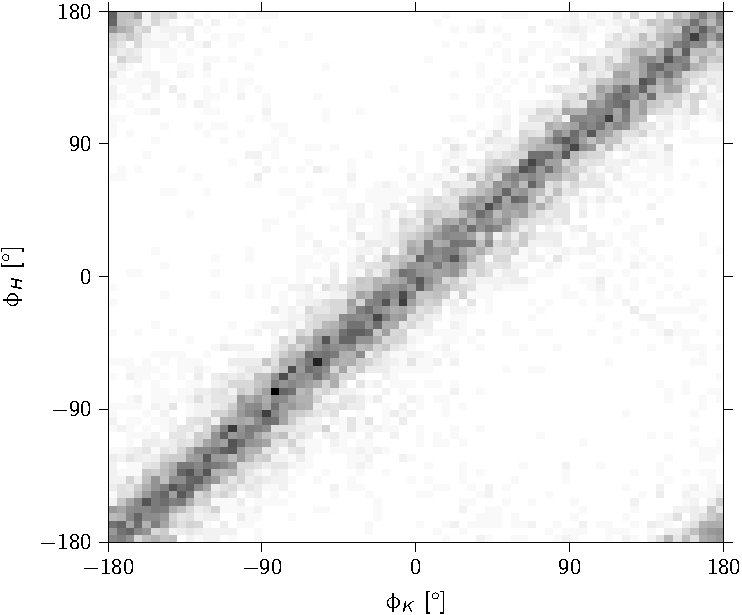
\includegraphics[width=0.4\textwidth]
                    {plots/experiment/azimuth_kascade_minn1}
    \caption{Angle reconstruction compared to KASCADE.}
    \label{fig:azimuth_kascade}
\end{figure}


\section{Network}
\label{sec:network-design}

- subsets of stations (same geographical region) are referred to as clusters.
- station data needs to be combined
- data sent over internet to Nikhef
    - per station data processed
    - coincidences between stations determined
- reason for GPS
    - station position
    - gps timestamps


\missingfigure{Dataflow infrastructure.}

\begin{figure}
    \centering
    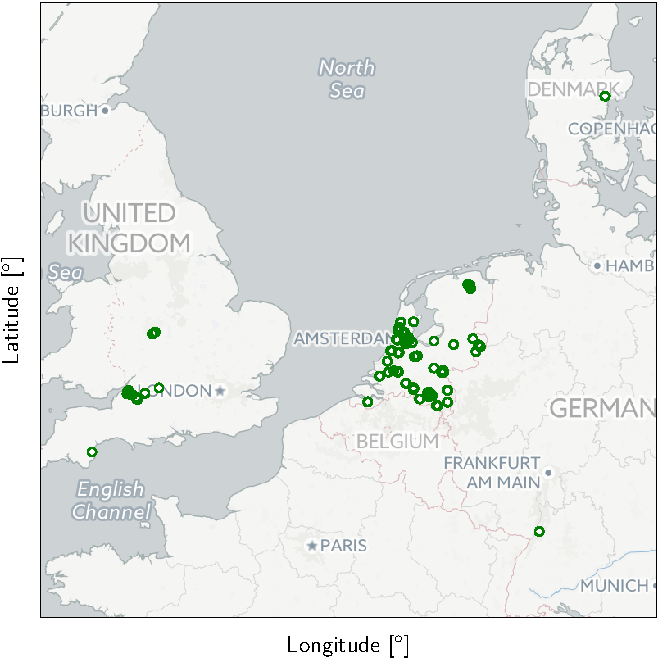
\includegraphics[width=0.4\textwidth]{plots/experiment/network}
    \caption{Map of station locations in the entire \hisparc network (Netherlands/England/Denmark).}
    \label{fig:network-map}
\end{figure}

\begin{figure}
    \centering
    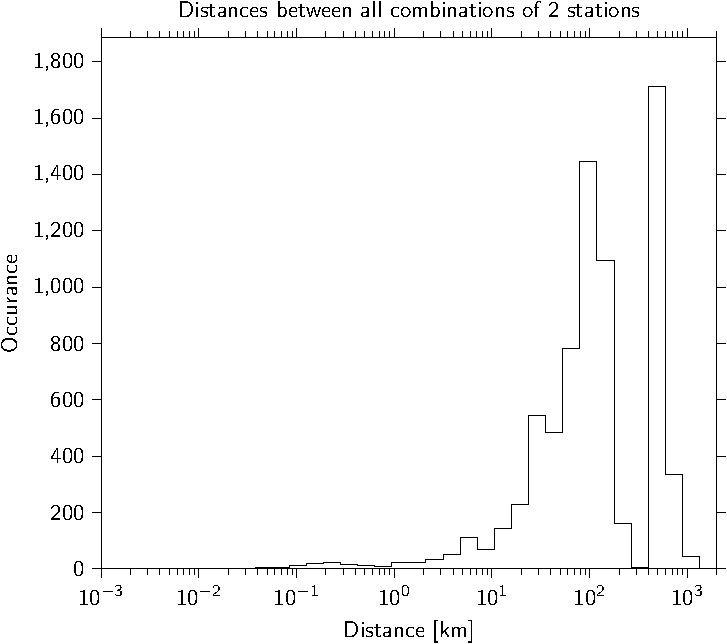
\includegraphics[width=0.6\textwidth]
                    {plots/experiment/network_station_distances}
    \caption{Distribution of distances between all station pairs.}
    \label{fig:network-distances}
\end{figure}


\begin{figure}
    \centering
    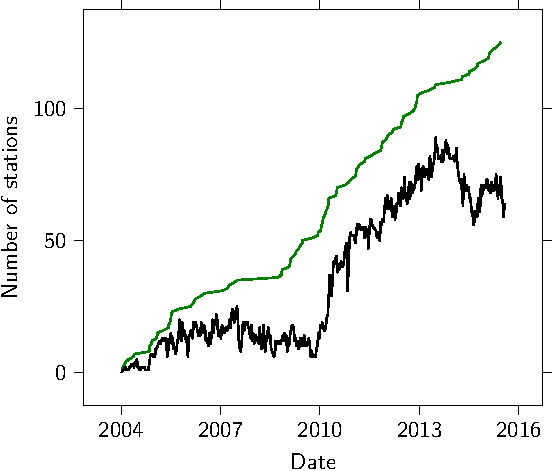
\includegraphics[width=0.45\textwidth]
                    {plots/experiment/active_stations}
    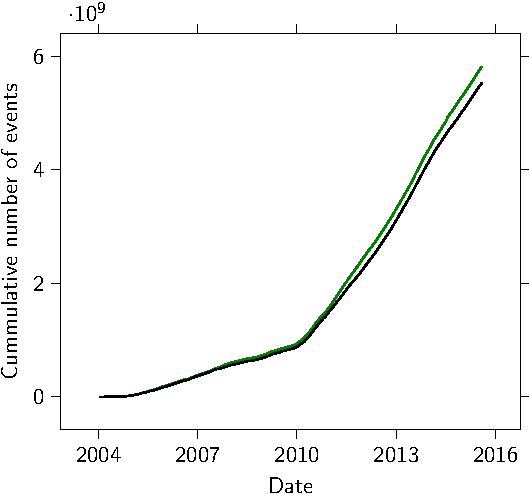
\includegraphics[width=0.45\textwidth]
                    {plots/experiment/luminosity_network}
    \caption{Total number of stations with data, number of stations active prer day. Total number of events and total number of good events.}
    \label{fig:active-luminosity}
\end{figure}



\subsection{Coincidences}

Accuracy of timestamps and effect of coincidence window
\missingfigure{GPS resolution/offsets.}

\begin{figure}
    \centering
    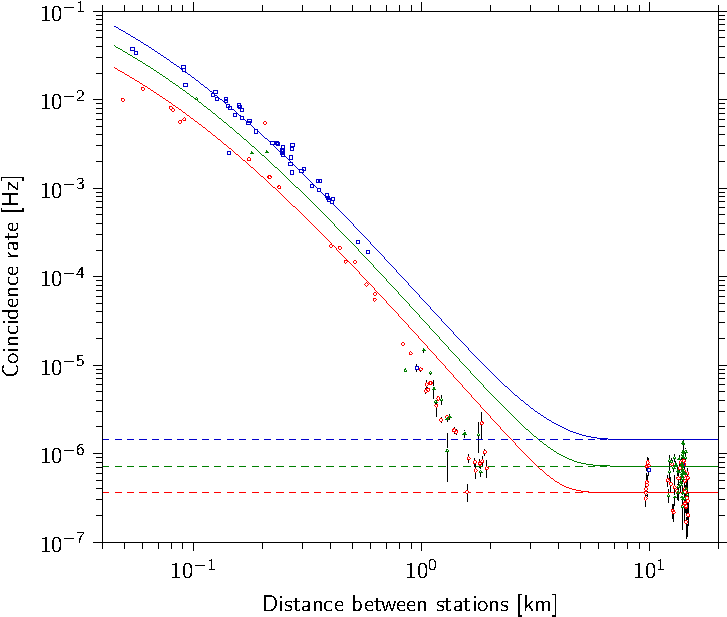
\includegraphics[width=0.6\textwidth]
                    {plots/experiment/distance_v_coincidence_rate}
    \caption{Coincidence rate between station pairs as a function of their distance, the different symbols indicate the number of detectors in the combination. The square indicates two 4-detector stations, triangle for a 4- and 2-detector station, and the circle two 2-detector stations. The dashed lines indicate the expected background rates. The solid lines the expected rates for the different combinations.}
    \label{fig:network-distances}
\end{figure}


\subsection{International}

Locations of \hisparc stations are not limited to the Netherlands.

In Germany one of our stations (70001) was placed inside the \kascade experiment in Karlsruhe on July 1, 2008. This was done to calibrate and test the direction reconstruction accuracy of a single \hisparc station. Although the \kascade-GRANDE \cite{kascade:grande} experiment officially shut down on March 30, 2009, it was kept active until November, 26th 2011 as a test facility for some test setups, including our detection station. The \kascade experiment \cite{kascade:experiment} triggered the \hisparc station when it detected a shower. It was triggered more than \num{9e7} (in publicdb, more on external hdd? and in `/databases/kascade`?) times in this period. The detectors used for the \kascade station have been repurposed and are now part of station 508 on the Science Park.

Since 2007 there has been a \hisparc station in Denmark. There are currently 3 operational stations at the Aarhus University. These stations are managed by Uffe Amelung Fredens. Fredens is writing student materials for Danish high school students.

In Bristol, United Kingdom a new cluster started to form in March 2012. This was initiated by Dr. Jaap Velthuis who is the cluster coordinator for the Bristol cluster. Since then schools around Bristol have joined the network. More on the way..

In 2014? a second cluster has started in the United Kingdom around Birmingham. The Birmingham cluster is coordinated by Cristina Lazzeroni.
